\chapter{Implementation}\label{ch:implementation}

In this chapter, we discuss the implementation of the system according to the
proposed architecture. The user application is described in
Section~\ref{sec:user_app}, the validator application in
Section~\ref{sec:validator_app}, and the smart contracts in
Section~\ref{sec:smart_contracts}, along with the tools required for deploying
the system. Although the user and validator applications are discussed in
separate sections, we have implemented a single application that serves both
roles in this project. However, in a real-world scenario, these would typically
be developed as separate applications.

\section{User App}\label{sec:user_app}

The user application serves as the primary interface for users to interact with
the system. Through this app, users can authenticate, browse events, and manage
their tickets. The app features a homepage for event browsing, an
event-specific page where users can view details and purchase tickets, and a
dedicated page to manage owned tickets. This section is structured as follows:
authentication is covered in Section~\ref{subsec:authentication}, event
browsing in Section~\ref{subsec:events}, and ticket management in
Section~\ref{subsec:tickets}.

The app is developed using the Flutter framework, a popular cross-platform
solution by Google that allows us to build applications for both Android and
iOS from a single codebase. Flutter is known for its ease of use and high
performance, making it well-suited for this project.

\subsection{Authentication}\label{subsec:authentication}

Figure~\ref{fig:authentication_page} shows the starting point of the app that
separates the authentication of the common users from the validators.

\begin{figure}[H]
	\centering
	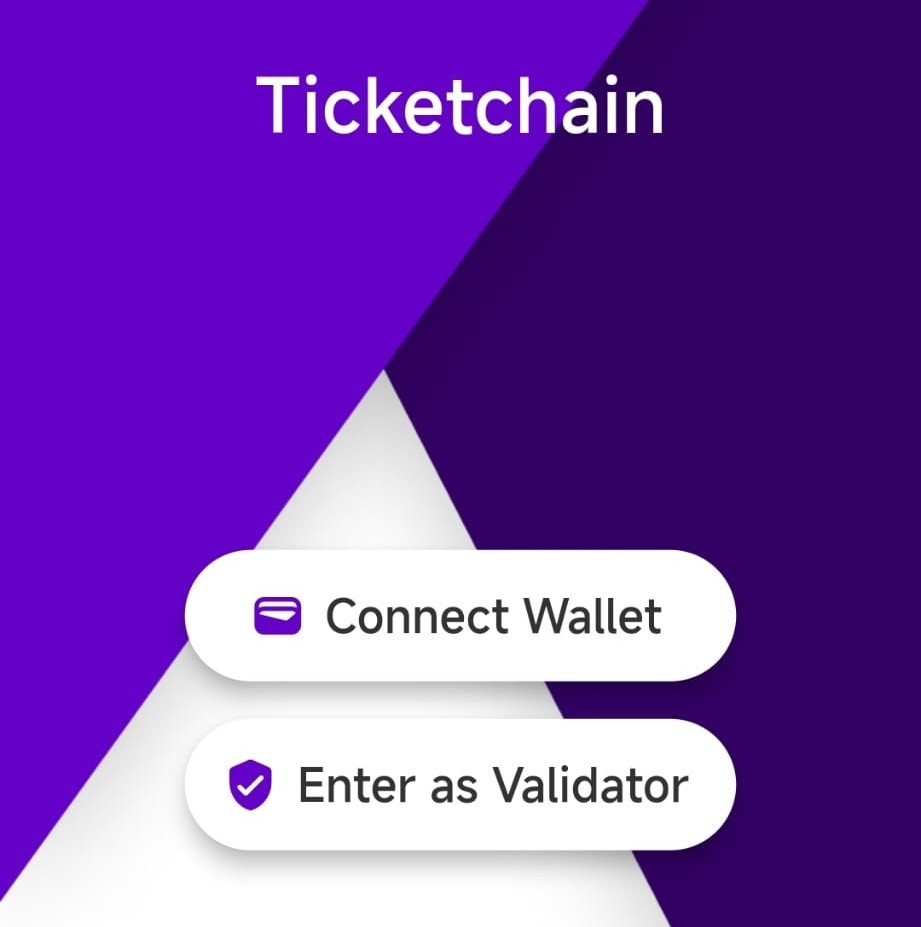
\includegraphics[width=\textwidth/3,frame]{Authentication page.jpg}
	\caption{Authentication page}\label{fig:authentication_page}
\end{figure}

To authenticate users, we use the Wallet Connect service~\cite{wallet_connect},
which supports a variety of wallets for user interaction. This service
establishes a secure connection between the app and a wallet, enabling the
wallet to receive prompts and sign transactions.

Figure~\ref{fig:wallet_connect_prompt} illustrates the Wallet Connect interface
that appears when users attempt to authenticate. This prompt displays all the
supported wallets, allowing the user to choose their preferred option.

\begin{figure}[H]
	\centering
	\includegraphics[width=\textwidth/3,frame]{Wallet connect prompt.jpg}
	\caption{Wallet Connect prompt}\label{fig:wallet_connect_prompt}
\end{figure}

Once a wallet is selected, the corresponding wallet app will automatically
open, and the user must approve the connection, as shown in
Figure~\ref{fig:metamask_connect}. For this implementation, we use
MetaMask~\cite{metamask}, a popular blockchain wallet. Users simply need to
create a MetaMask wallet to begin interacting with the app.

\begin{figure}[H]
	\centering
	\includegraphics[width=\textwidth/3,frame]{Metamask connect.jpg}
	\caption{MetaMask connection approval}\label{fig:metamask_connect}
\end{figure}

The authentication is a one-time process, so the user doesn't have to do this
every time he wants to interact with the app. Basically when a connection is
established, the next time the app tries to reconnect to the wallet, it will
skip the prompt.

\subsection{Events}\label{subsec:events}

After the common user authenticates, he will be redirected to the home page of
the app, shown in Figure~\ref{fig:home_page}, where he can see the events that
are available.

\begin{figure}[H]
	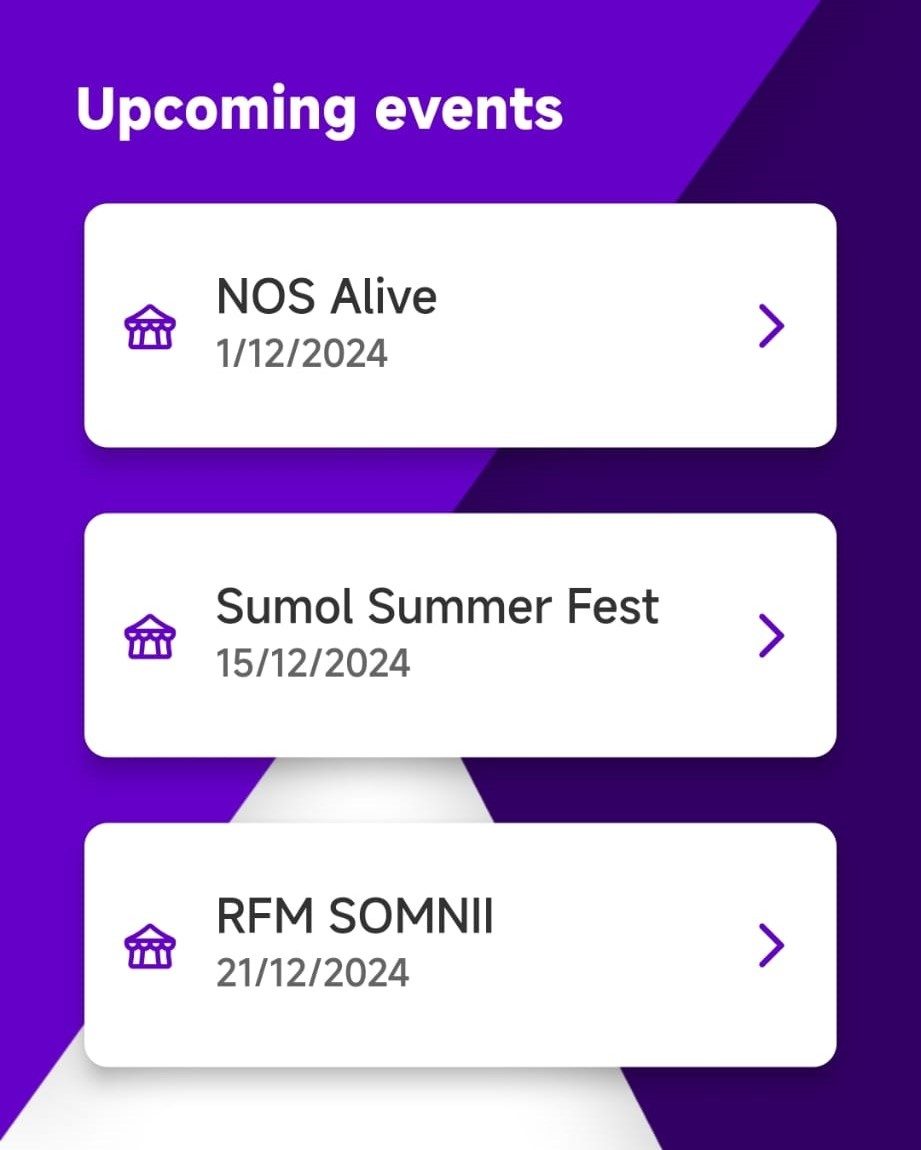
\includegraphics[width=\textwidth/3,frame]{Home page.jpg}
	\centering
	\caption{Home page}\label{fig:home_page}
\end{figure}

When clicking in one of the events, the user will be redirected to the event
page. Figure~\ref{fig:event_page} shows the event page, where the user can see
the details of the event and the packages available.

\begin{figure}[H]
	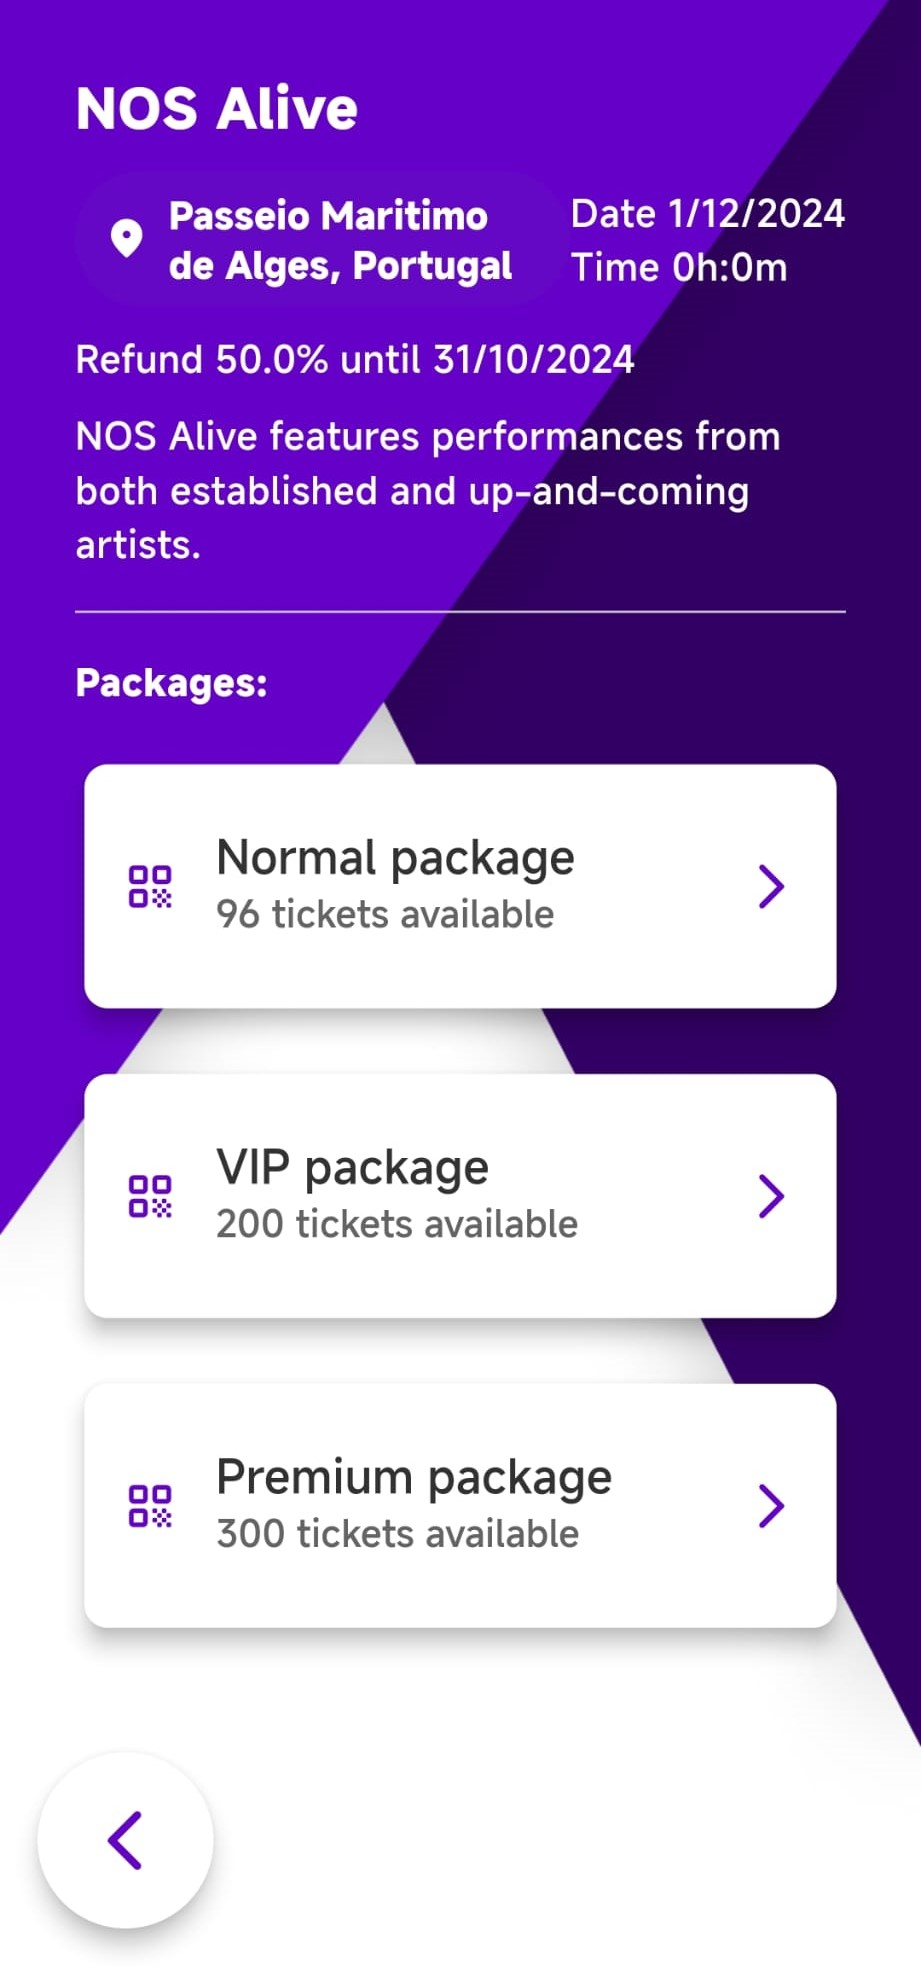
\includegraphics[width=\textwidth/3,frame]{Event page.jpg}
	\centering
	\caption{Event page}\label{fig:event_page}
\end{figure}

The user sees the name, description, location, date, packages and even the
refund information. When the user taps on the package he wants to buy, the
prompt shown in Figure~\ref{fig:buy_tickets_prompt} shows up, where the user
can choose the amount of tickets he wants to buy. We went with this approach of
only choosing the amount of tickets to buy, but in the future a feature like
seat selection could be implemented.

\begin{figure}[H]
	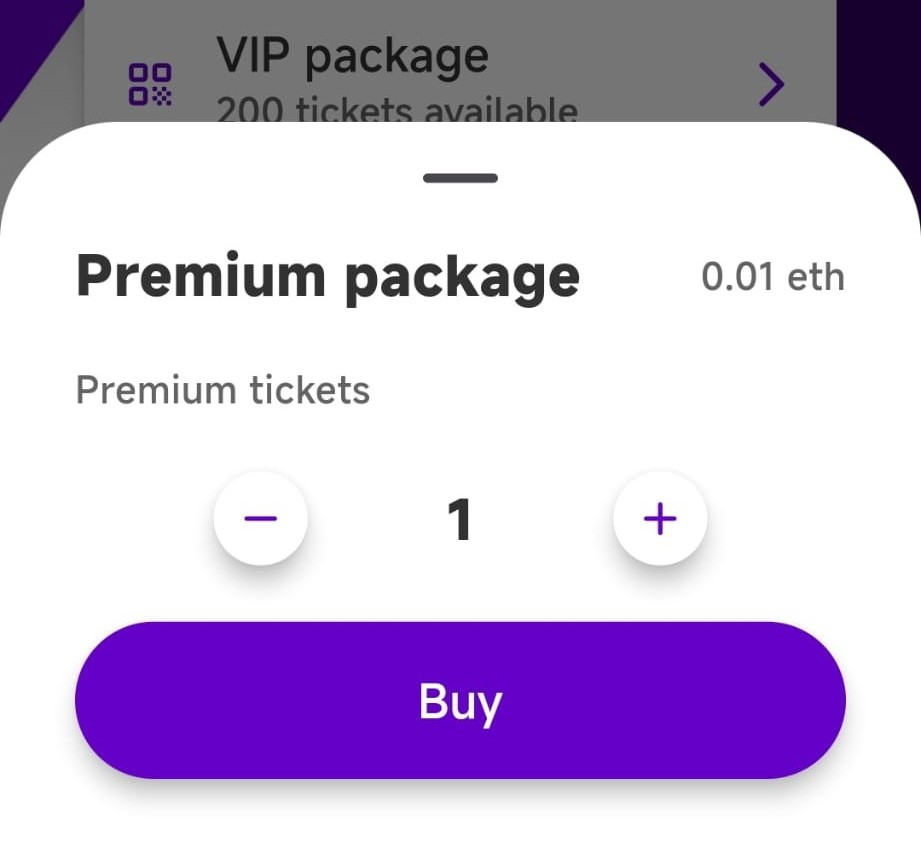
\includegraphics[width=\textwidth/3,frame]{Buy tickets prompt.jpg}
	\centering
	\caption{Buy tickets prompt}\label{fig:buy_tickets_prompt}
\end{figure}

The user can then confirm the purchase, and the wallet will prompt the user to
sign the transaction, as shown in the
Figure~\ref{fig:metamask_transaction_prompt}. It displays the amount of money
the user has to pay, to which address he's interacting with, and the total cost
to execute the transaction.

\begin{figure}[H]
	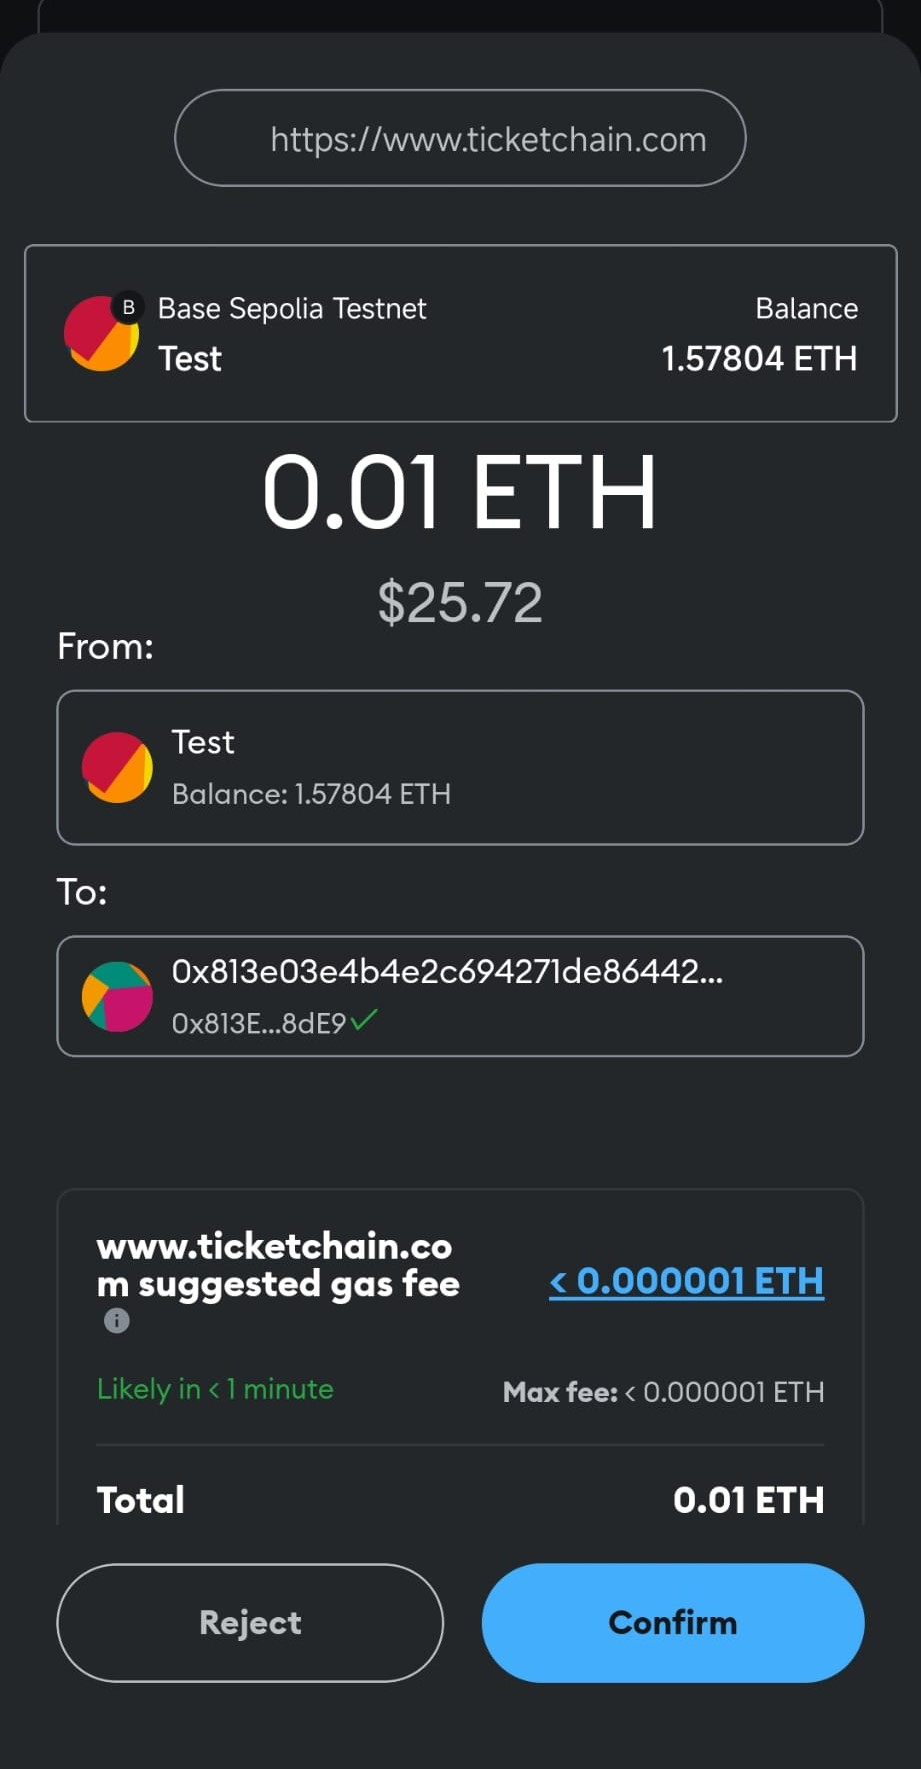
\includegraphics[width=\textwidth/3,frame]{MetaMask transaction prompt.jpg}
	\centering
	\caption{MetaMask transaction prompt}\label{fig:metamask_transaction_prompt}
\end{figure}

\subsection{Tickets}\label{subsec:tickets}

After confirmation, the user is redirected back to the app where, on the second
tab with the profile icon, the profile page, he will be able to see the events
which he owns any tickets, as shown in Figure~\ref{fig:profile_page}.

\begin{figure}[H]
	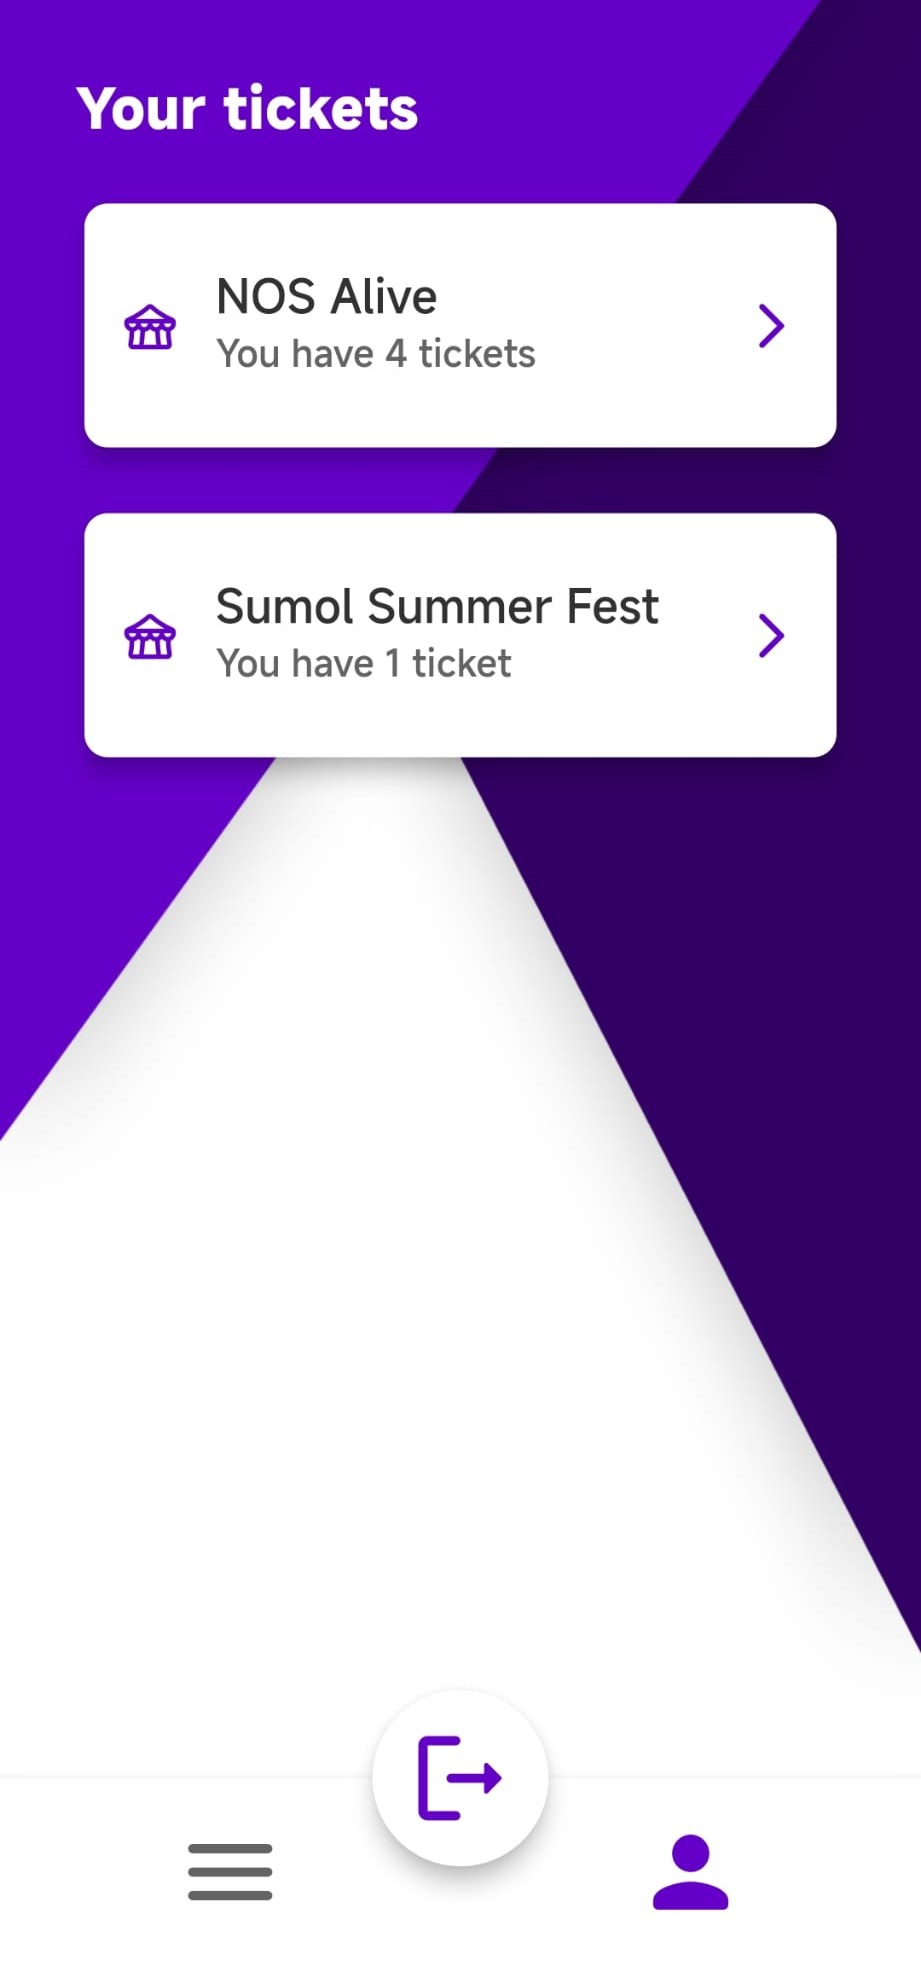
\includegraphics[width=\textwidth/3,frame]{Profile page.jpg}
	\centering
	\caption{Profile page}\label{fig:profile_page}
\end{figure}

Going into one of them, like Figure~\ref{fig:tickets_page} shows, the user can
see the tickets he owns for that event. It's a similar page as the normal event
one, but with the tickets he owns instead of the packages available. We see 4
tickets here and the first one has a mark on it, which means the ticket has
already been validated.

\begin{figure}[H]
	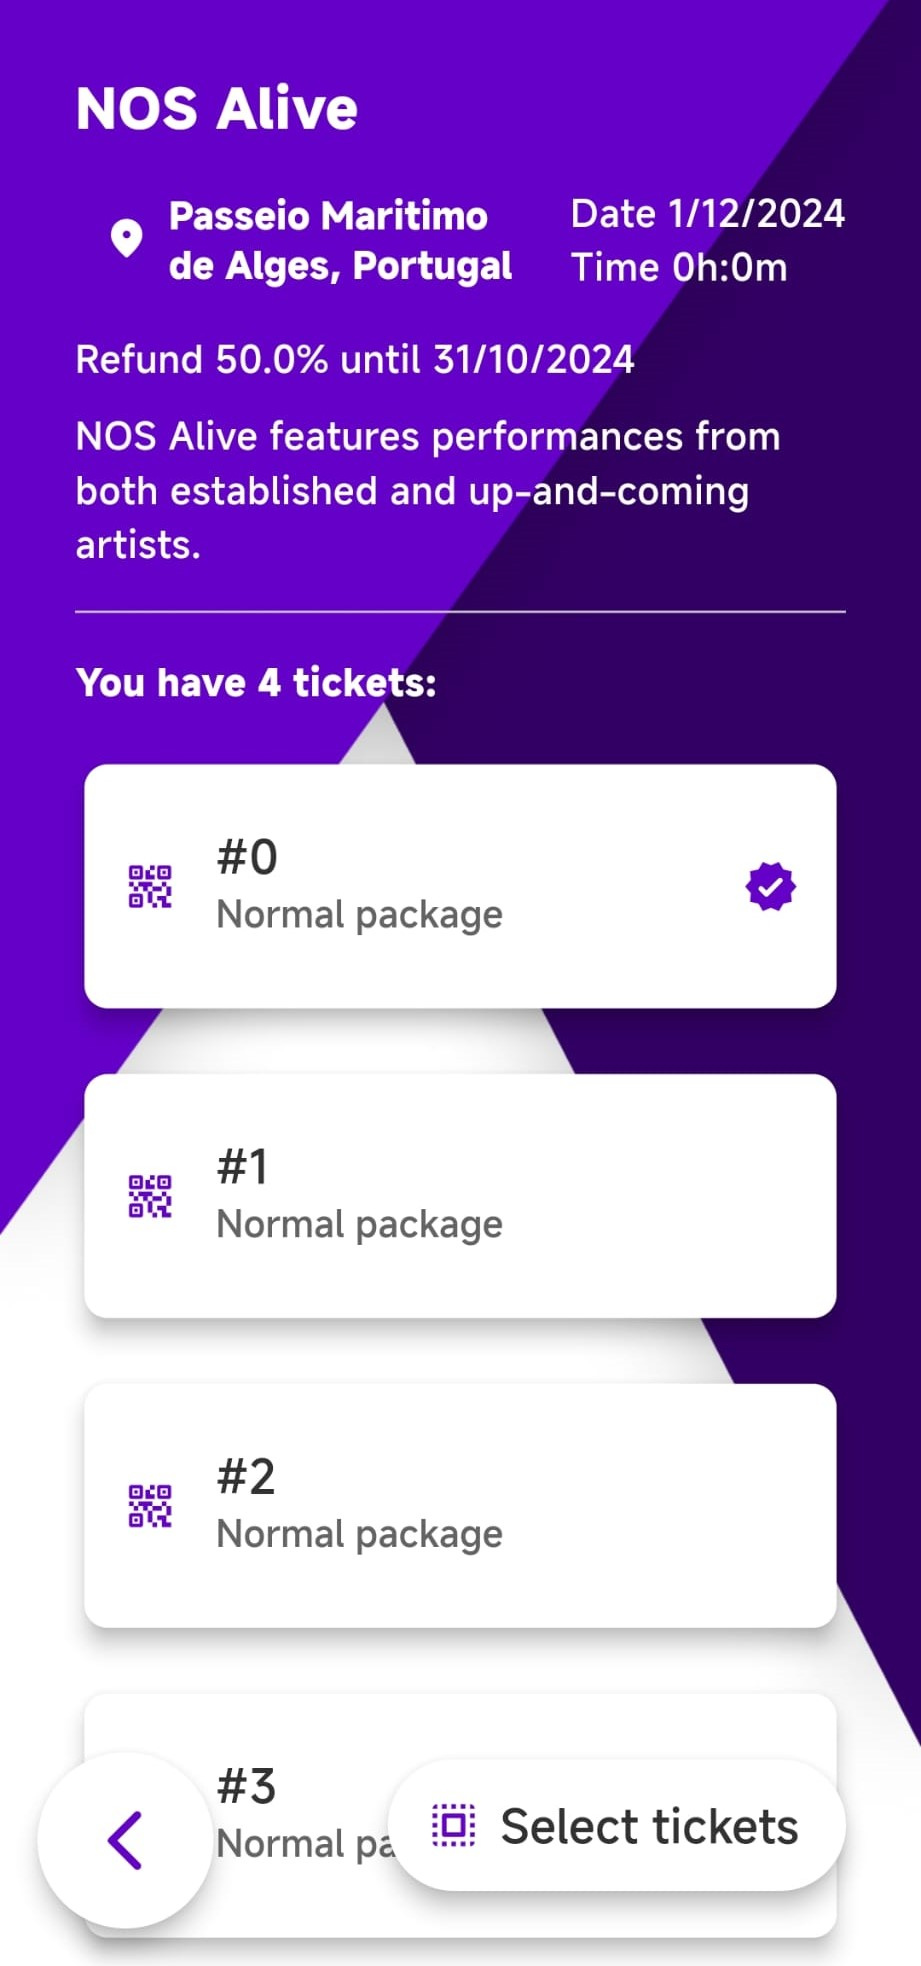
\includegraphics[width=\textwidth/3,frame]{Tickets page.jpg}
	\centering
	\caption{Tickets page}\label{fig:tickets_page}
\end{figure}

Clicking on one of the tickets, it shows us the basic ticket information, along
with its image, as shown in Figure~\ref{fig:ticket_information}.

\begin{figure}[H]
	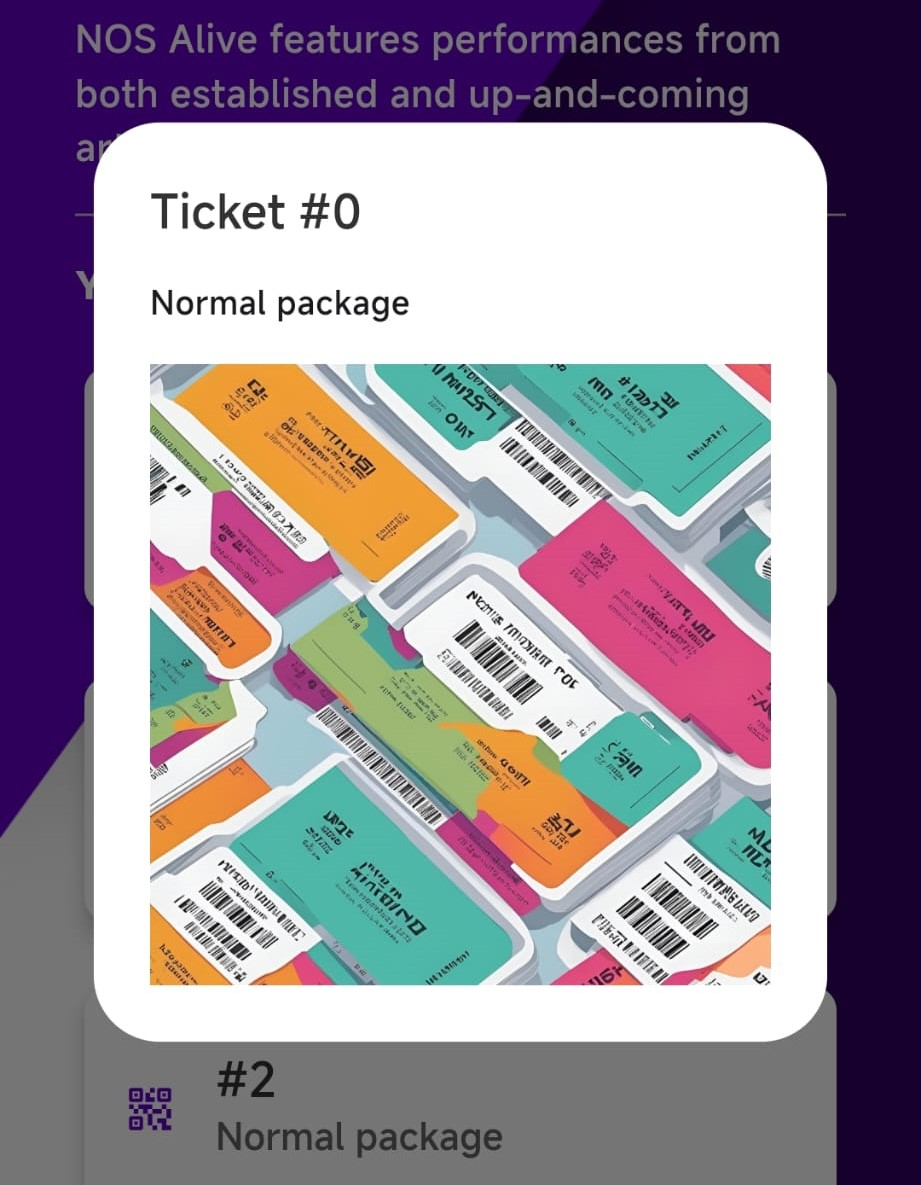
\includegraphics[width=\textwidth/3,frame]{Ticket information.jpg}
	\centering
	\caption{Ticket information}\label{fig:ticket_information}
\end{figure}

For operating the tickets, the user can simply click on the select tickets
button which will allow him to choose the tickets which he wishes to operate,
as shown in Figure~\ref{fig:ticket_operations}. In this case the user sees only
3 tickets (while Figure~\ref{fig:tickets_page} shows 4) because since the first
is already validated, it's not possible to operate on it anymore. We see the
options to gift, refund and validate the tickets he selected.

\begin{figure}[H]
	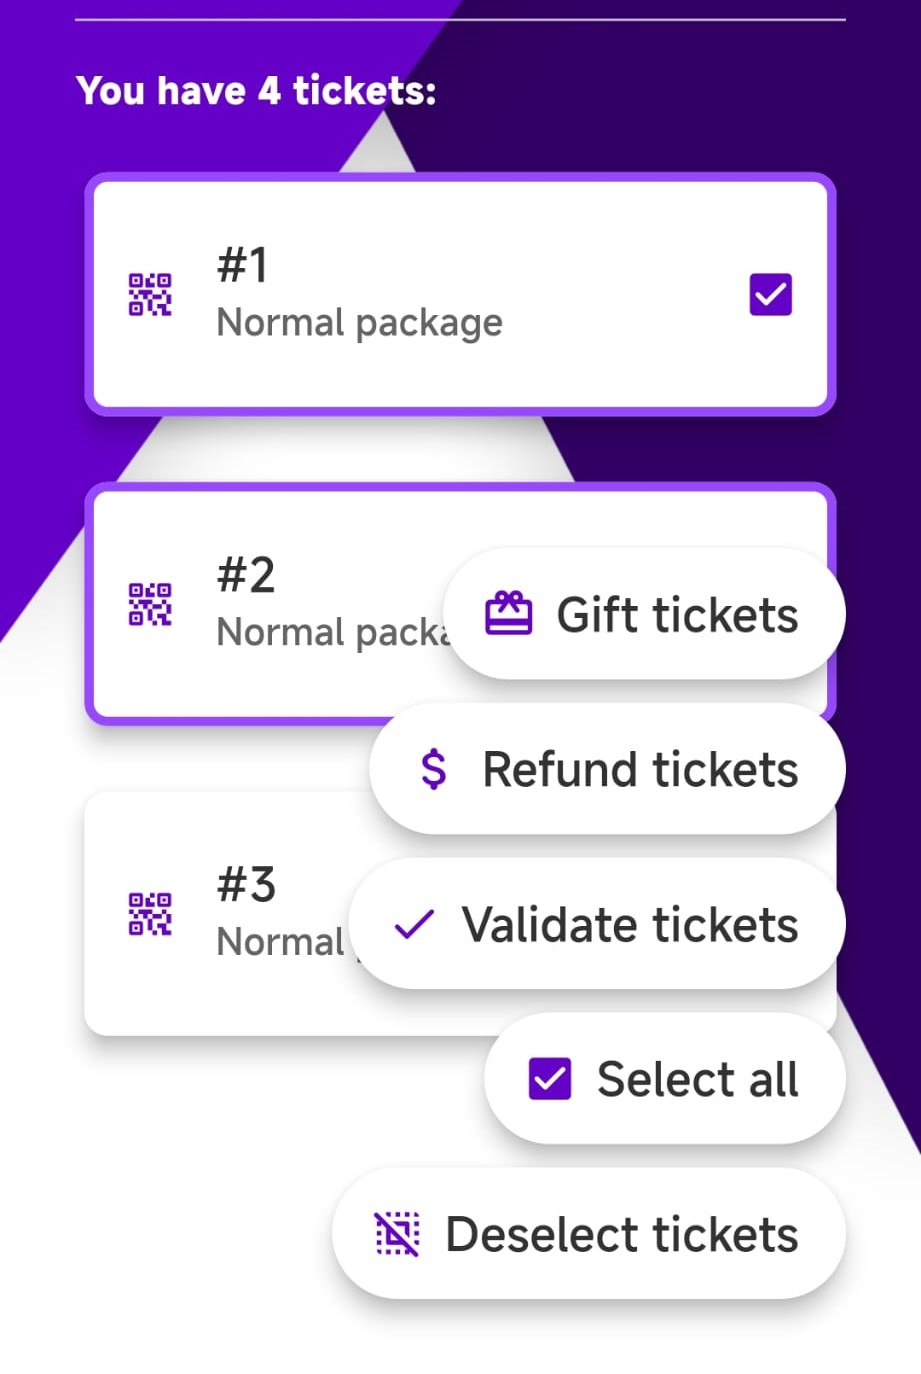
\includegraphics[width=\textwidth/3,frame]{Ticket operations.jpg}
	\centering
	\caption{Ticket operations}\label{fig:ticket_operations}
\end{figure}

The gift option will ask the user for the address to which he wants to gift the
tickets. After that, it will trigger the wallet to sign the transaction, and
the tickets will be transferred to the address.

The refund option will ask the user to confirm the refund, and trigger the
wallet to confirm the transaction in which the tickets will be burned, making
them available again for other users to buy, and returning the correct amount
of money to the user.

The validate option will start the validation process, which will be explained
in the Section~\ref{subsec:validate_tickets}.

\section{Validator App}\label{sec:validator_app}

For the validator app, we will have a simple interface for the validators to
execute the validation process. Like mentioned, this is currently done in the
same app as the common users, but in a real scenario we would have a separate
app for the validators.

Ideally we will authenticate the same way as common users, but for the sake of
making it easy to demonstrate and test, the app will behave as a wallet.
Essentially this means that the app holds the private keys and signs the
transactions.

This section is divided in two: the validator address in
Section~\ref{fig:validator_address} and the ticket validation in
Section~\ref{subsec:validate_tickets}.

\subsection{Validator Address}\label{subsec:validator_address}

Since this is the case, we need a way to see the address of the validator, so
that the organizer can add him to the event and give him the necessary funds to
operate. The reason for the necessary funds is mentioned in the
Section~\ref{subsubsec:system_fees}.

The Figure~\ref{fig:validator_page} shows the starting point of the app after
authentication, where the validator has the option to check the address and to
validate the tickets.

\begin{figure}[H]
	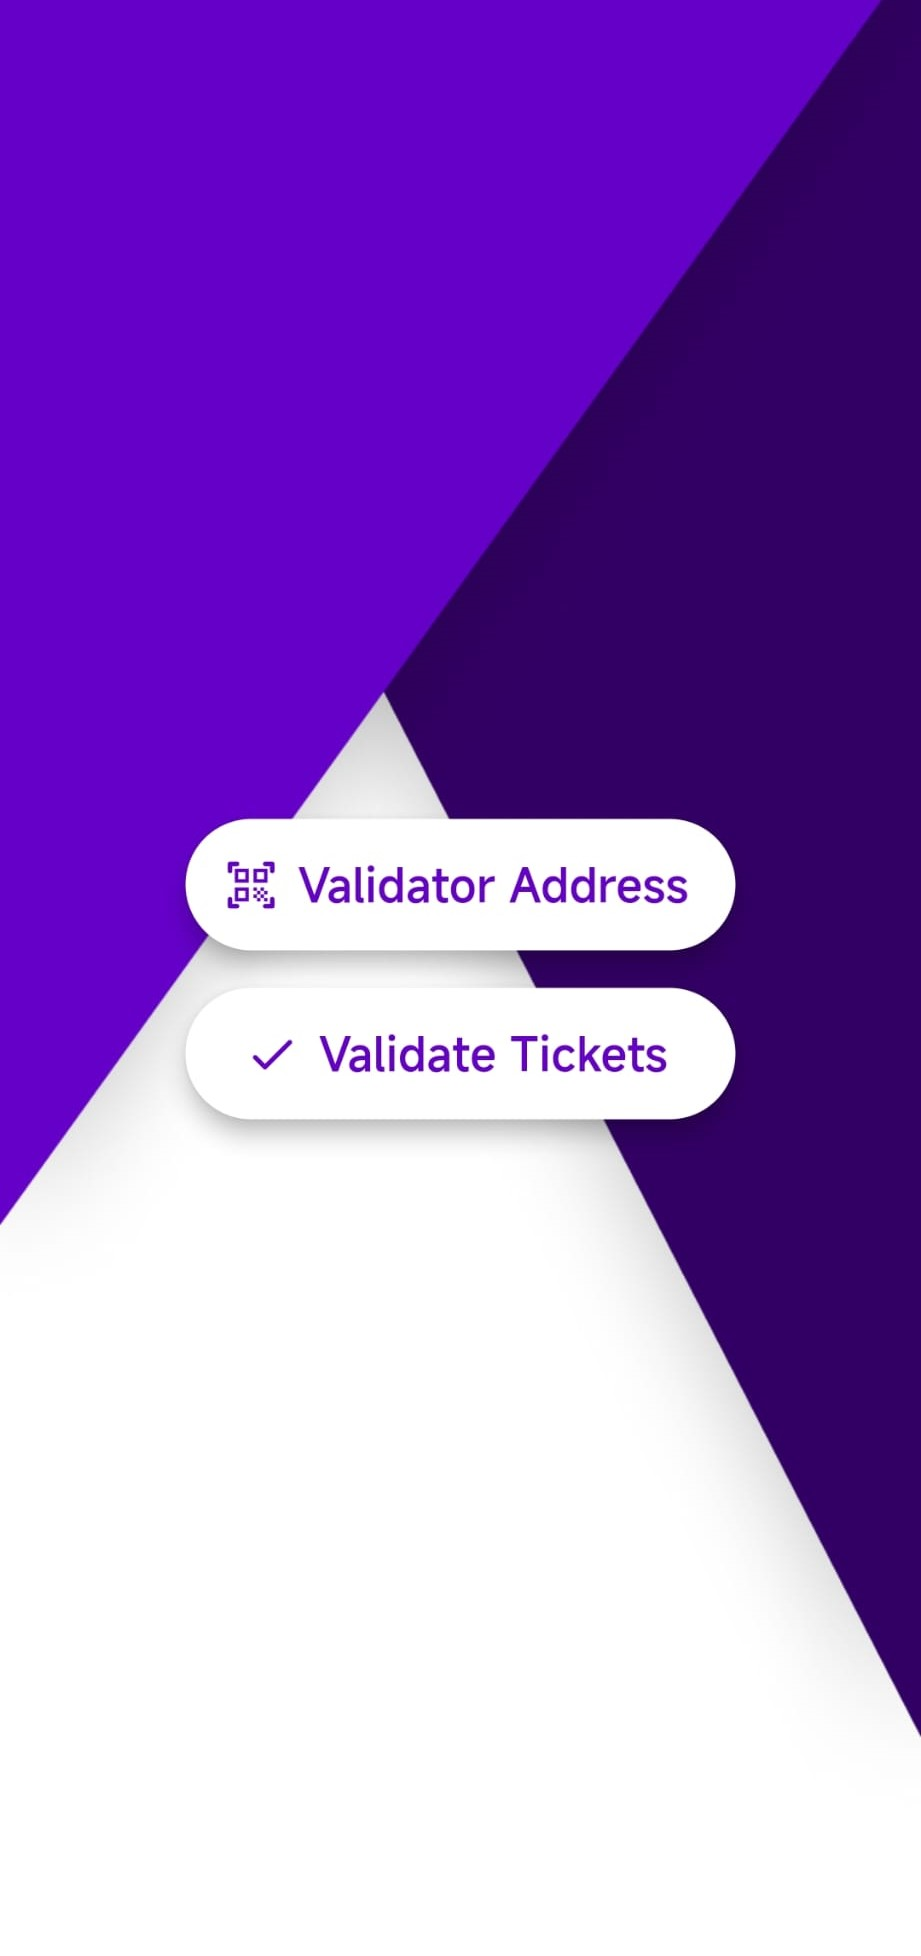
\includegraphics[width=\textwidth/3,frame]{Validator page.jpg}
	\centering
	\caption{Validator page}\label{fig:validator_page}
\end{figure}

When the validator taps the address he will see his address, as well as its QR
code, as shown in Figure~\ref{fig:validator_address}.

\begin{figure}[H]
	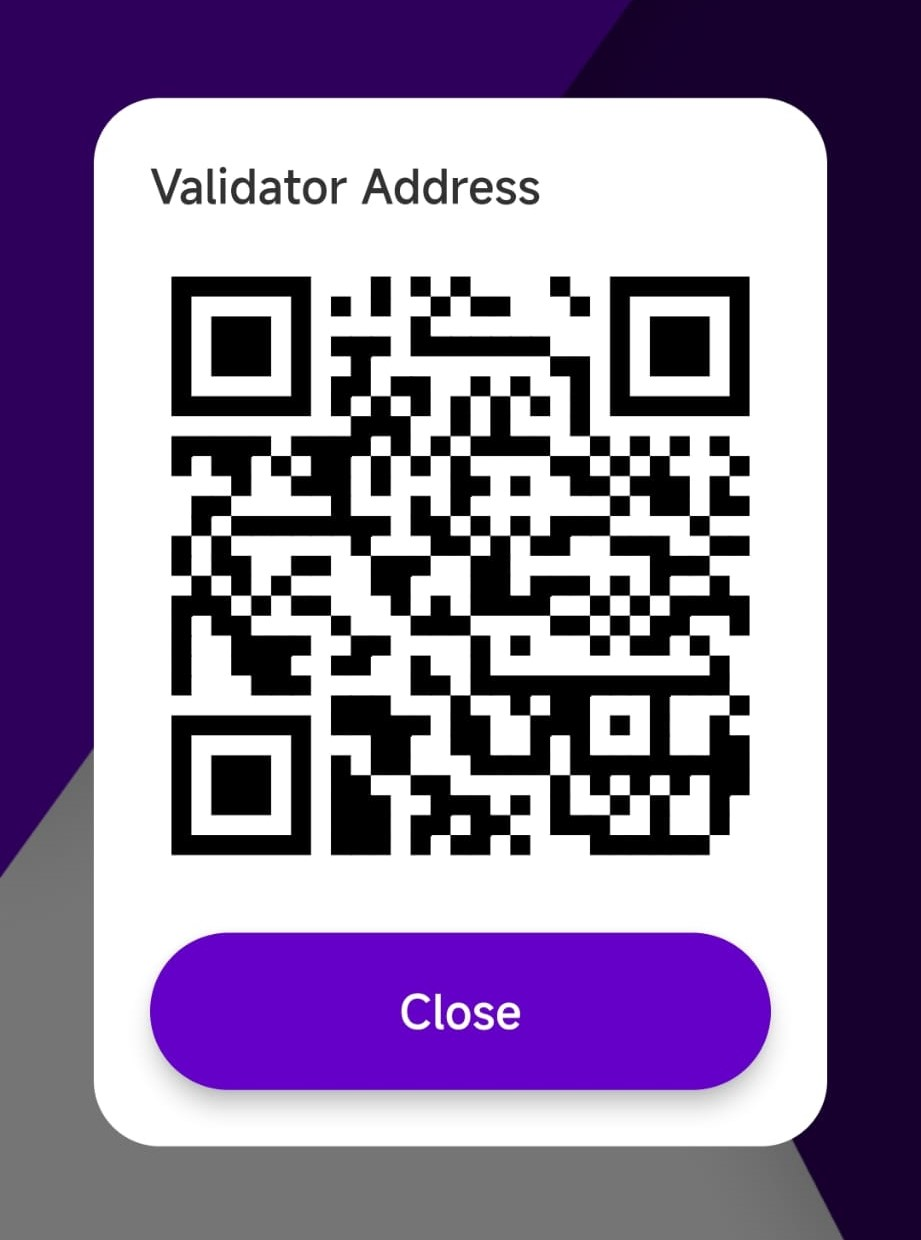
\includegraphics[width=\textwidth/3,frame]{Validator address.jpg}
	\centering
	\caption{Validator address}\label{fig:validator_address}
\end{figure}

When the validator select the validate tickets option, he will start the
process of validating the tickets, which will be explained in the next
Section~\ref{subsec:validate_tickets}.

\subsection{Validate Tickets}\label{subsec:validate_tickets}

For the ticket validation process, we must take into consideration a lot of
aspects, because it's not just checking if the user address has a ticket
associated to him. This is because, since the data is on the blockchain and
it's public, anyone can see the addresses where each ticket belongs to, and
pretend he's the owner of the ticket. For this to be secure, we need to
guarantee the user is actually the owner of the address, and here is where the
cryptographic message signature comes in, the same process that happens when
executing a blockchain transaction, which needs the user to sign the
transaction, proving he's allowed to execute the transaction.

We came up with the process shown in Figure~\ref{fig:ticket_validation}, that
shows the steps between the actors and the system to validate the tickets.

\begin{figure}[H]
	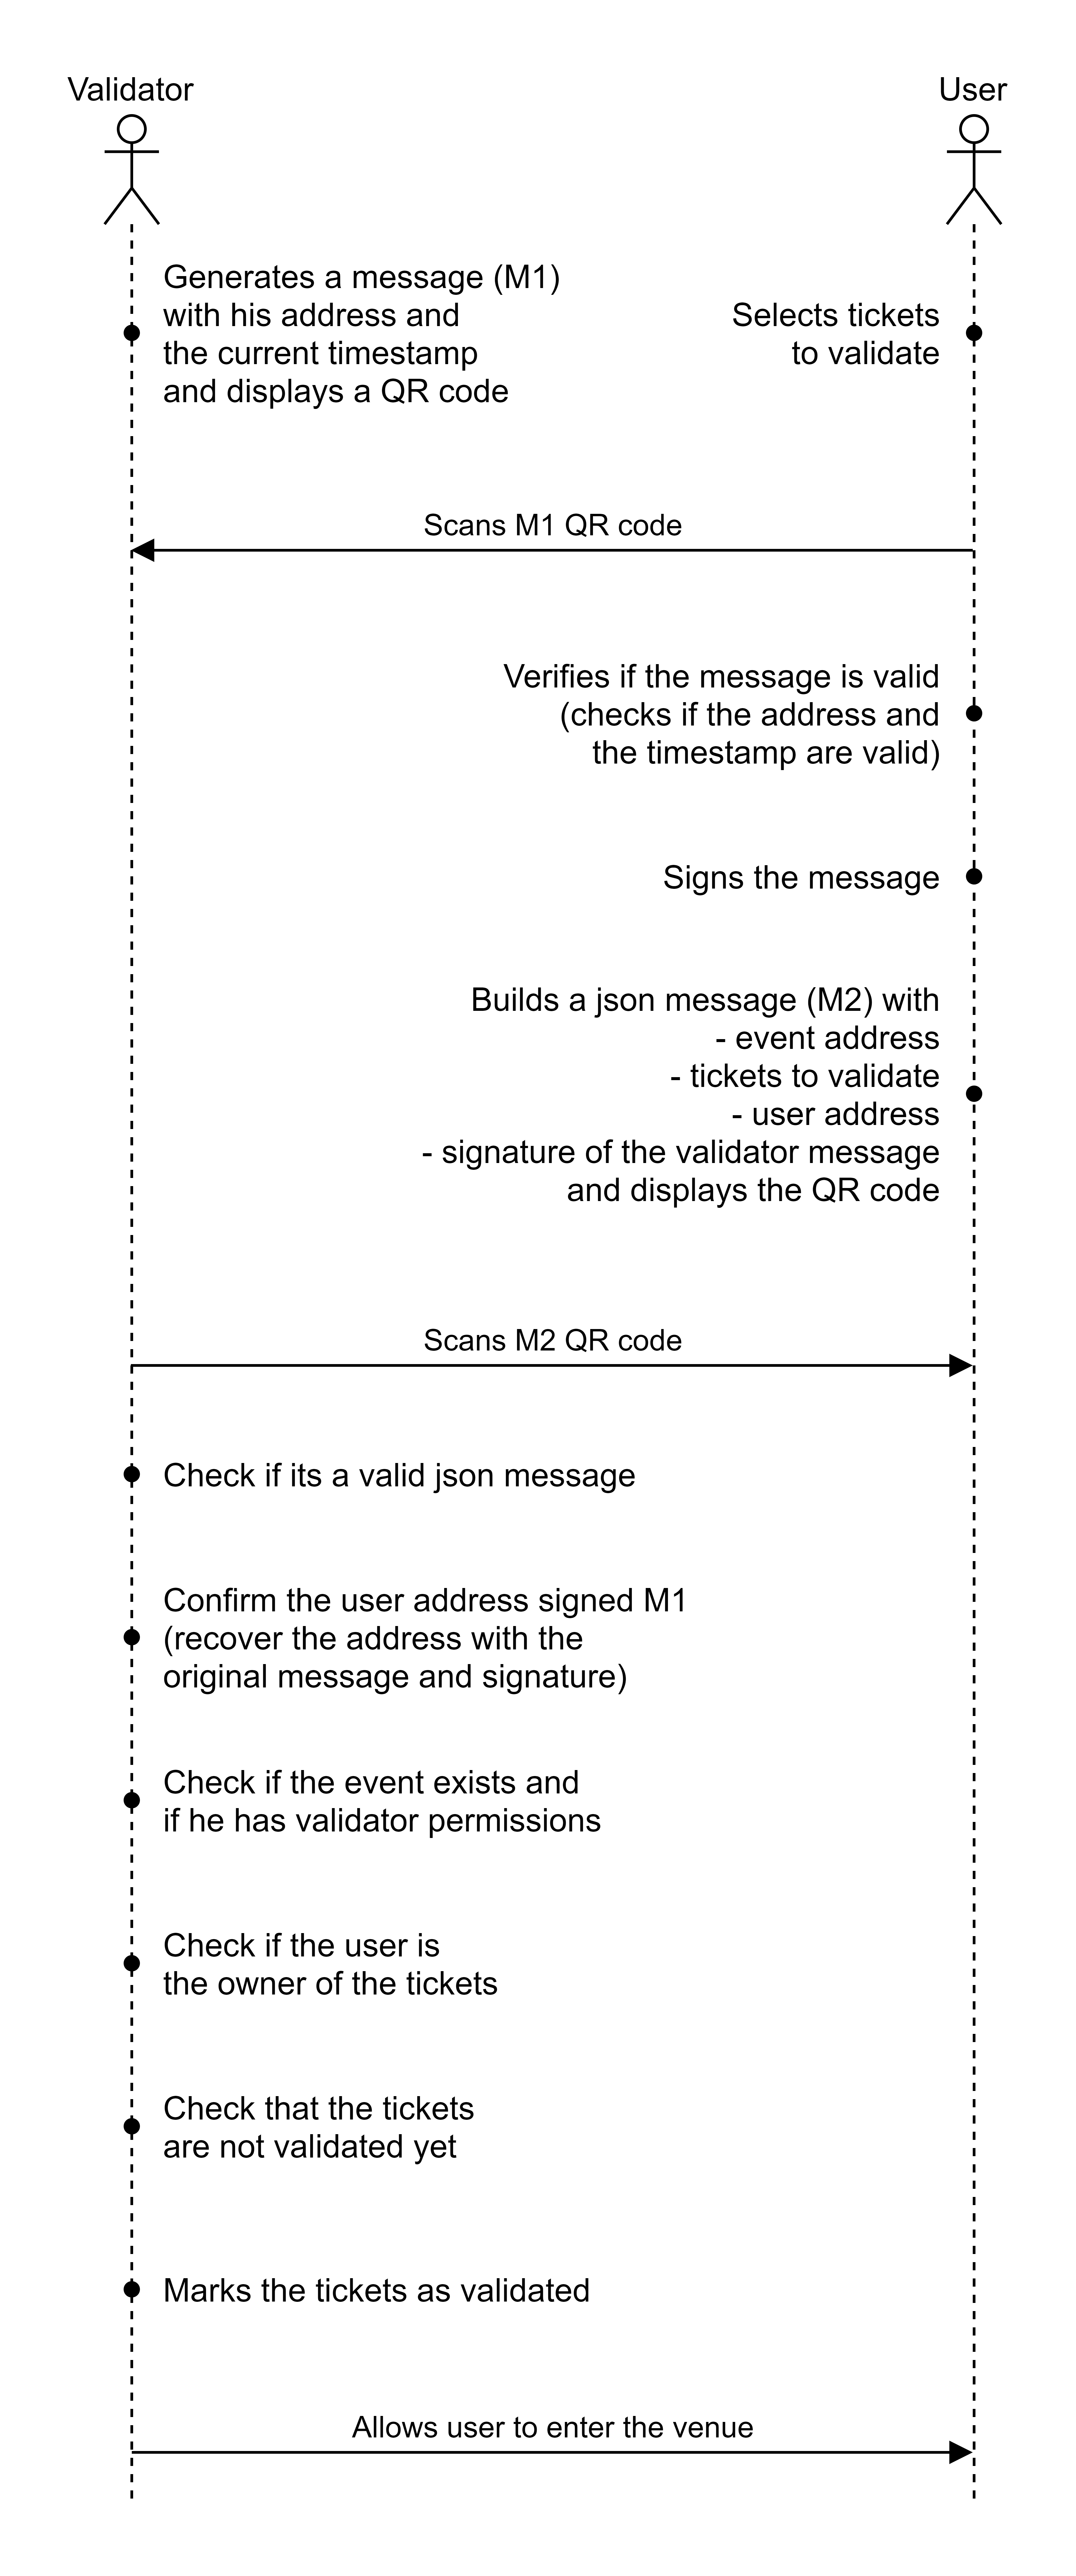
\includegraphics[height=\textheight]{Ticket validation.png}
	\centering
	\caption{Ticket validation}\label{fig:ticket_validation}
\end{figure}

Here we see that the user reads the QR with a generated message from the
validator, then signs it with his wallet, and generates a JSON with the
signature and useful information like the tickets to validate, the event, and
the user address. After the validator reads the JSON in the QR code, he checks
if the parameters match the ones on the blockchain, gets the address using a
cryptographic method to recover it through the original message and it's
signature, and checks if the user is the owner of the tickets. If everything
matches, the validator will trigger a transaction to mark the tickets as
validated, to avoid people sharing the accounts and using the same ticket
multiple times.

Both parties need to know the original message, so it matches. We could just
use a default message for everyone, so the users would just need to give the
signature to the validator, but this could become a security issue in case the
signature gets leaked, because anyone who has it could pretend to be someone
else. The idea here is to have a unique message for each user at the time of
the event, so they are forced to sign it.

All this is reduced to a single transaction on the blockchain because,
depending on the network, the finality of a transaction (a term used in the
blockchain ecosystem that defines the time it takes for a transaction to be
fully registered) can take a while. This was planned to be done in a single
transaction to avoid congestion at the entrance of the venue, so the users can
enter the event with the least amount of delay. This is an important aspect to
consider when designing the system to fullfil the system being fast, so like
mentioned in the Section~\ref{subsec:non_functional_requirements}, the network
choice is crucial.

\section{Smart Contracts}\label{sec:smart_contracts}

We split this section into the main three contracts of the system: the
Ticketchain contract in Section~\ref{subsec:ticketchain_contract}, the ERC721
contract in Section~\ref{subsec:erc721_standard}, and the Event contract in
Section~\ref{subsec:event_contract}.

The deployment of the smart contracts will be done using
Foundry~\cite{foundry}, a toolkit for the development and deployment of the
smart contracts, which makes it easy to deploy to any network, and also to test
the contracts locally.

So smart contracts are similar to C++ mainly because it lies on a class-like
structure with variables to store data and methods, where the main difference
is that a class is called a contract. You can also extend others to integrate
their functionalities. That's essentially what's gonna happen with each event,
extending the ERC721 standard, making it a collection of NFTs, where each NFT
is a ticket.

Since this is the behavior we want (each event being a NFT collection), we will
have to deploy (instantiate, in C++) a new contract for each event, so we will
have a main contract (called Ticketchain, since it's the main contract) to keep
track of them. This structure can be visualized in the
Figure~\ref{fig:system_uml}, which shows the simplified \gls{uml} of the
system.

\begin{figure}[H]
	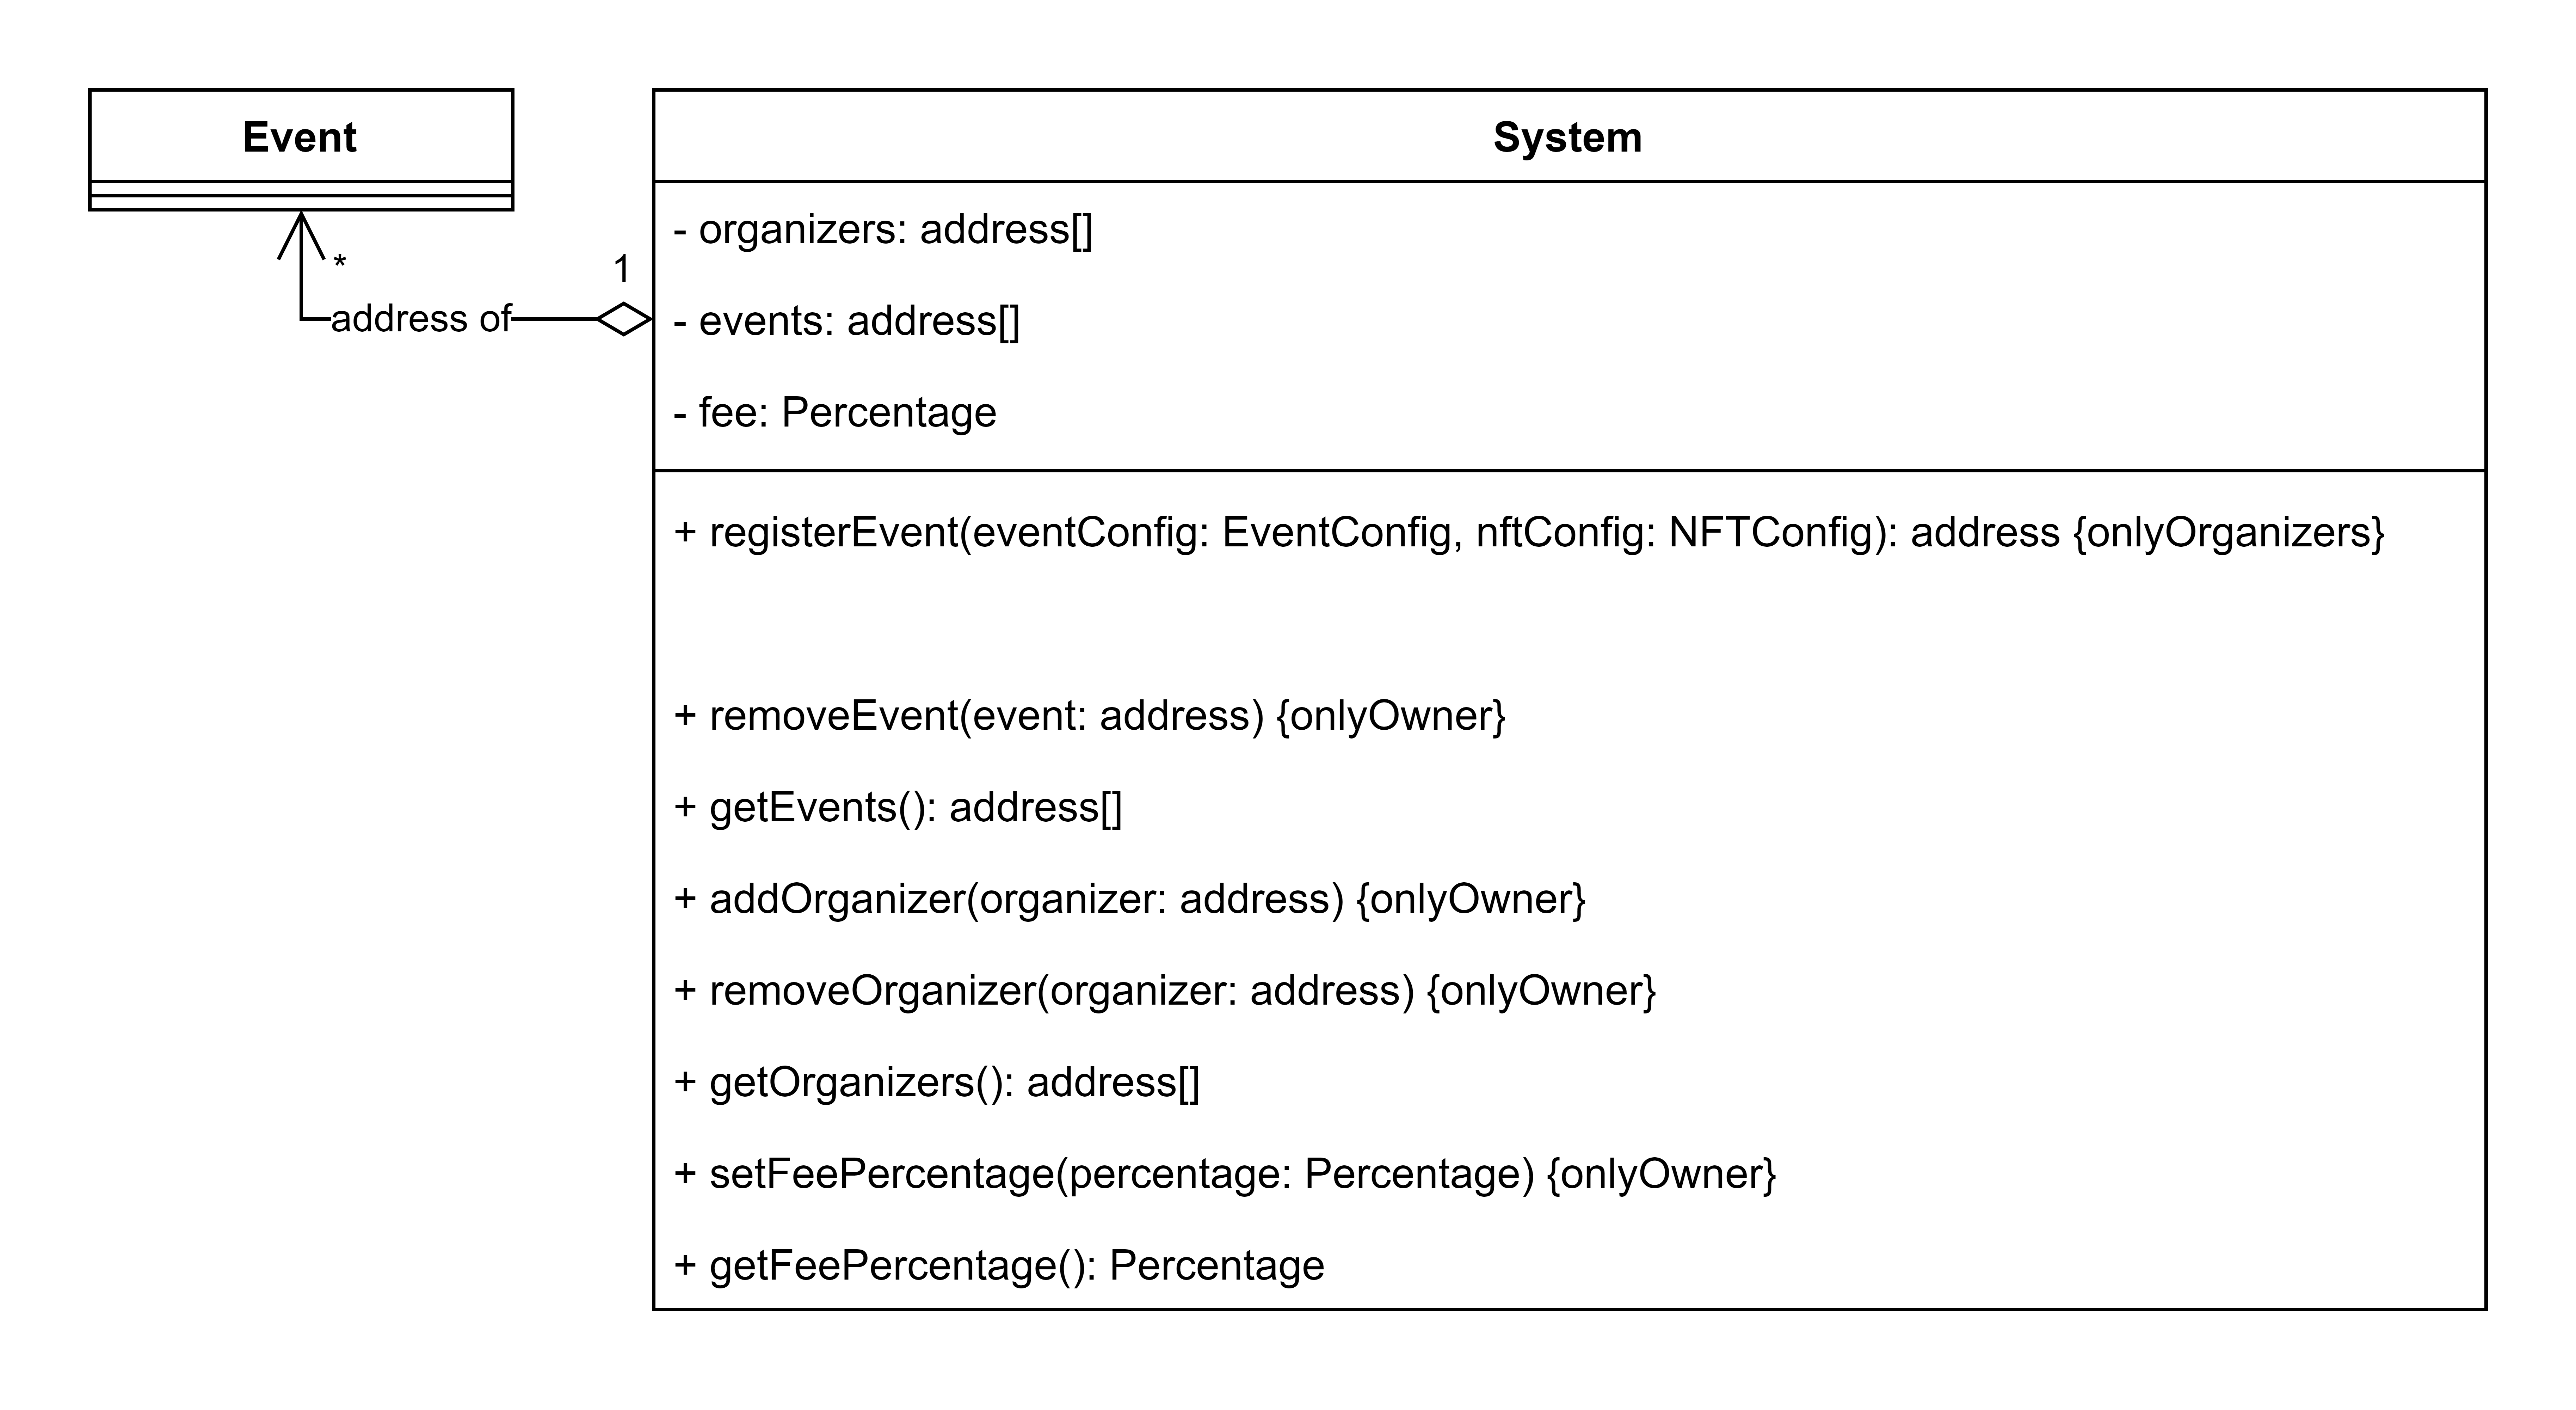
\includegraphics[width=\textwidth*2/3]{System UML.png}
	\centering
	\caption{System UML (simplified)}\label{fig:system_uml}
\end{figure}

We see that the Event contract extends the ERC721 standard, and the Ticketchain
contract will deploy the events and keep track of them. The contracts will be
explained in detail over the next sections.

\subsection{Ticketchain Contract}\label{subsec:ticketchain_contract}

The Ticketchain contract is the main contract of the system, from where the
events are registered and stored. It will have the necessary methods to
register new events and to add organizers. The Figure~\ref{fig:ticketchain_uml}
shows the most relevant methods of the contract.

\begin{figure}[H]
	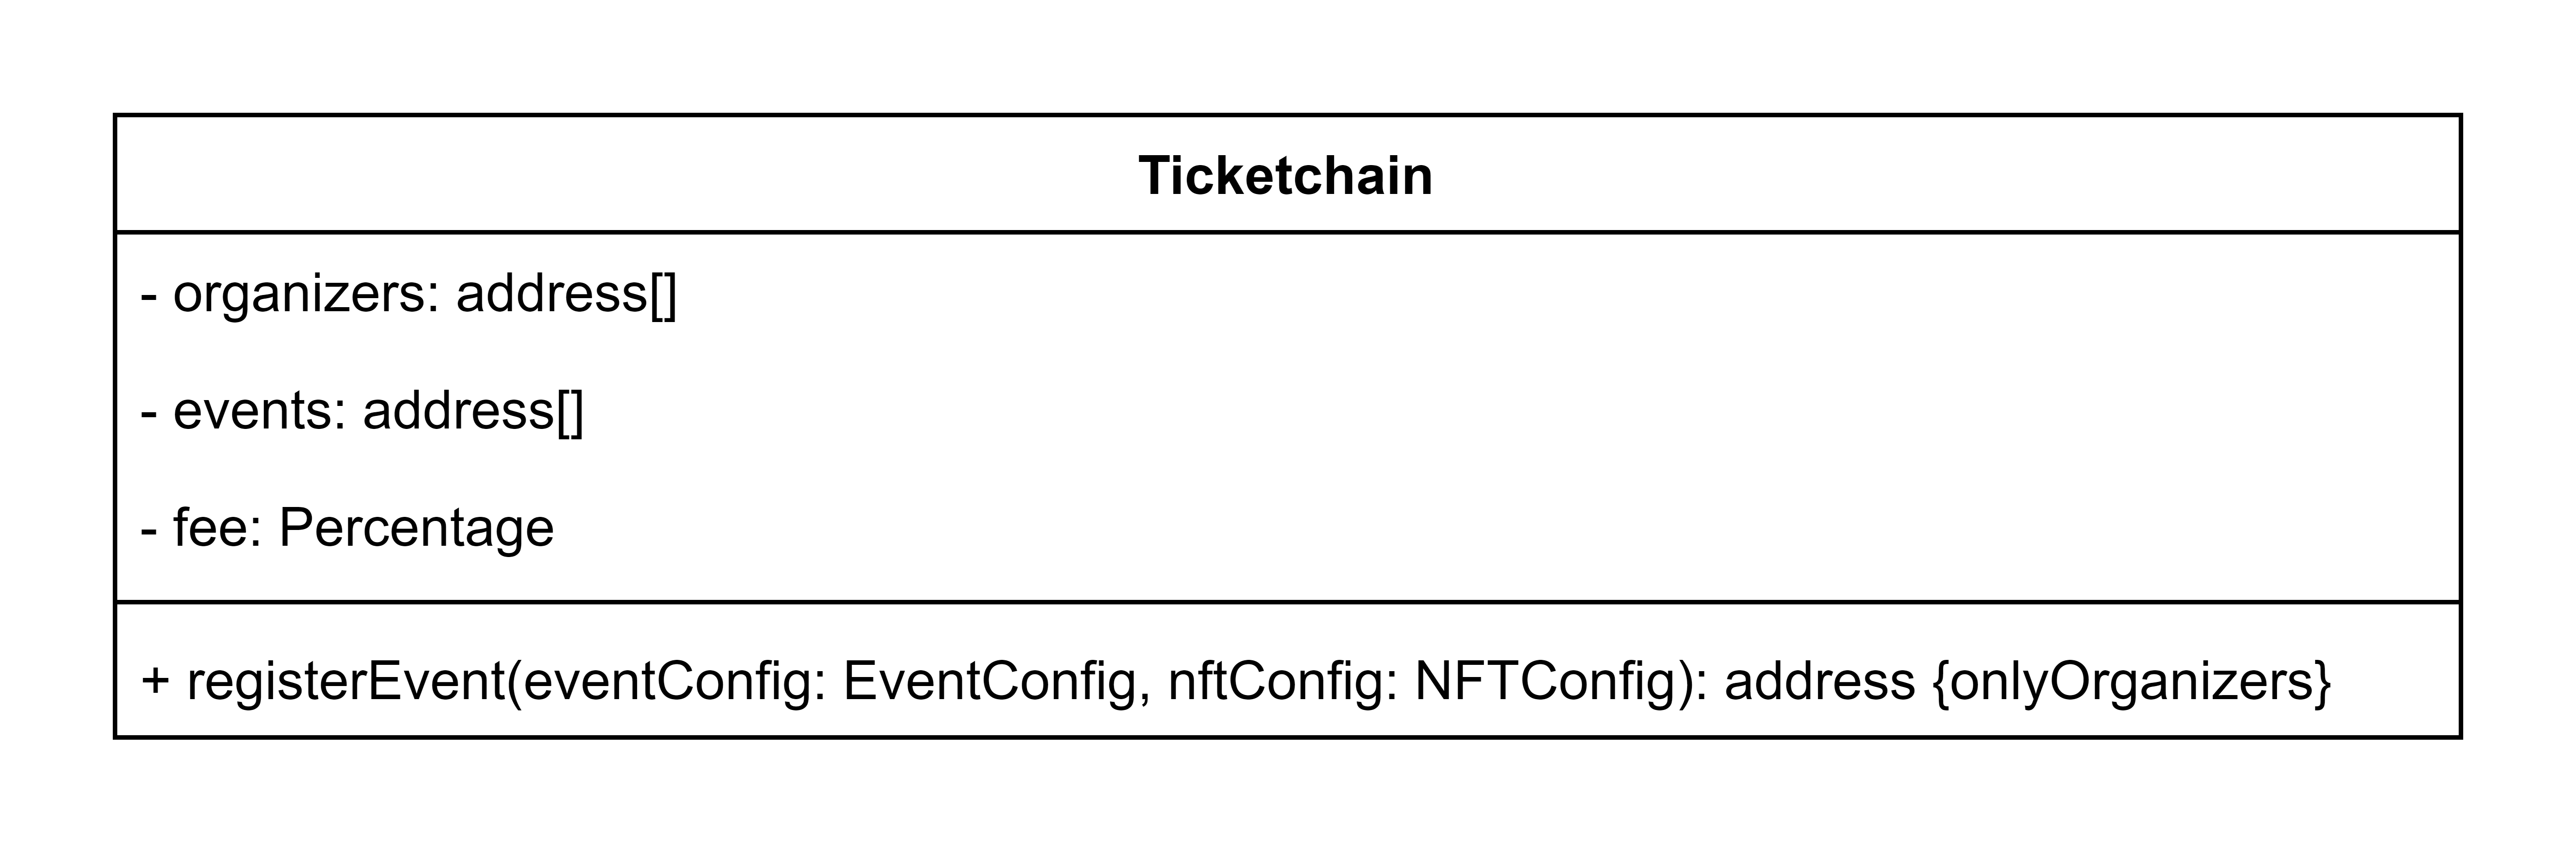
\includegraphics[width=\textwidth*2/3]{Ticketchain UML.png}
	\centering
	\caption{Ticketchain UML (relevant methods)}\label{fig:ticketchain_uml}
\end{figure}

We have method to add organizers, so only the ones that are allowed can create
events. This is a good feature to have because it prevents unauthorized people
to create events and possibly scam the users. The organizer is the one that
will be able to add the necessary information about the event, like the name,
description, location, dates, and packages, and also to manage the event, like
adding packages, changing the dates, and refunding the tickets.

When an event is created, we transfer the ownership of the event to the
organizer, so he can manage it. This is a common practice in the blockchain
ecosystem, where the ownership of the contract is transferred to the user that
created it, so he he's fully responsible for it. This ownership is restricted
by using modifiers that check if the user is the owner of the event, so only
the organizer can execute the necessary operations.

We also have the events address list, which is a way to track all the events
that are deployed, so we can easily get them all and show them in the app. The
fee variable is there to store the system fee, which will be mentioned in the
Section~\ref{subsubsec:system_fees}.

\subsection{ERC721 Standard}\label{subsec:erc721_standard}

The ERC721 standard will be extended and we will be adding the necessary
methods to interact with the tickets, like buying, selling, and validating
them. The reason to extend this standard and not implement the logic manually
is mainly because it makes it compatible with the most common marketplaces for
NFTs, which allows for users to do what they desire with them after the event.
It also has the necessary methods to manage the tickets, like transferring them
between users, and the necessary operations to track these operations.

The standard was obtained through the OpenZeppelin~\cite{openzeppelin} library,
which is a collection of secure and community-vetted smart contracts that are
used by many projects in the Ethereum ecosystem. This library is a great
resource for developers to build secure and reliable smart contracts.

Analyzing its source code~\cite{erc721_github}, and looking into the most
important variables and methods of the standard shown in
Figure~\ref{fig:erc721_uml}, we can understand that the NFTs are simply a
mapping of the token ID to the owner address, so when you execute a transaction
to get a token (this process is called minting), the token ID is then
associated to your address. Then for each token it's possible set a \gls{uri},
which is a link to the NFTs metadata, usually being a JSON file with the
necessary information about the token, like the name, description, and image.

This link could point to anything, for example a google drive file, but the
common thing is to store the metadata on the \gls{ipfs}~\cite{ipfs}, which is a
decentralized storage system, so the metadata is not stored on the blockchain
itself (onchain), which would be very expensive, but rather on a decentralized
storage system (offchain), which is much cheaper.

\begin{figure}[H]
	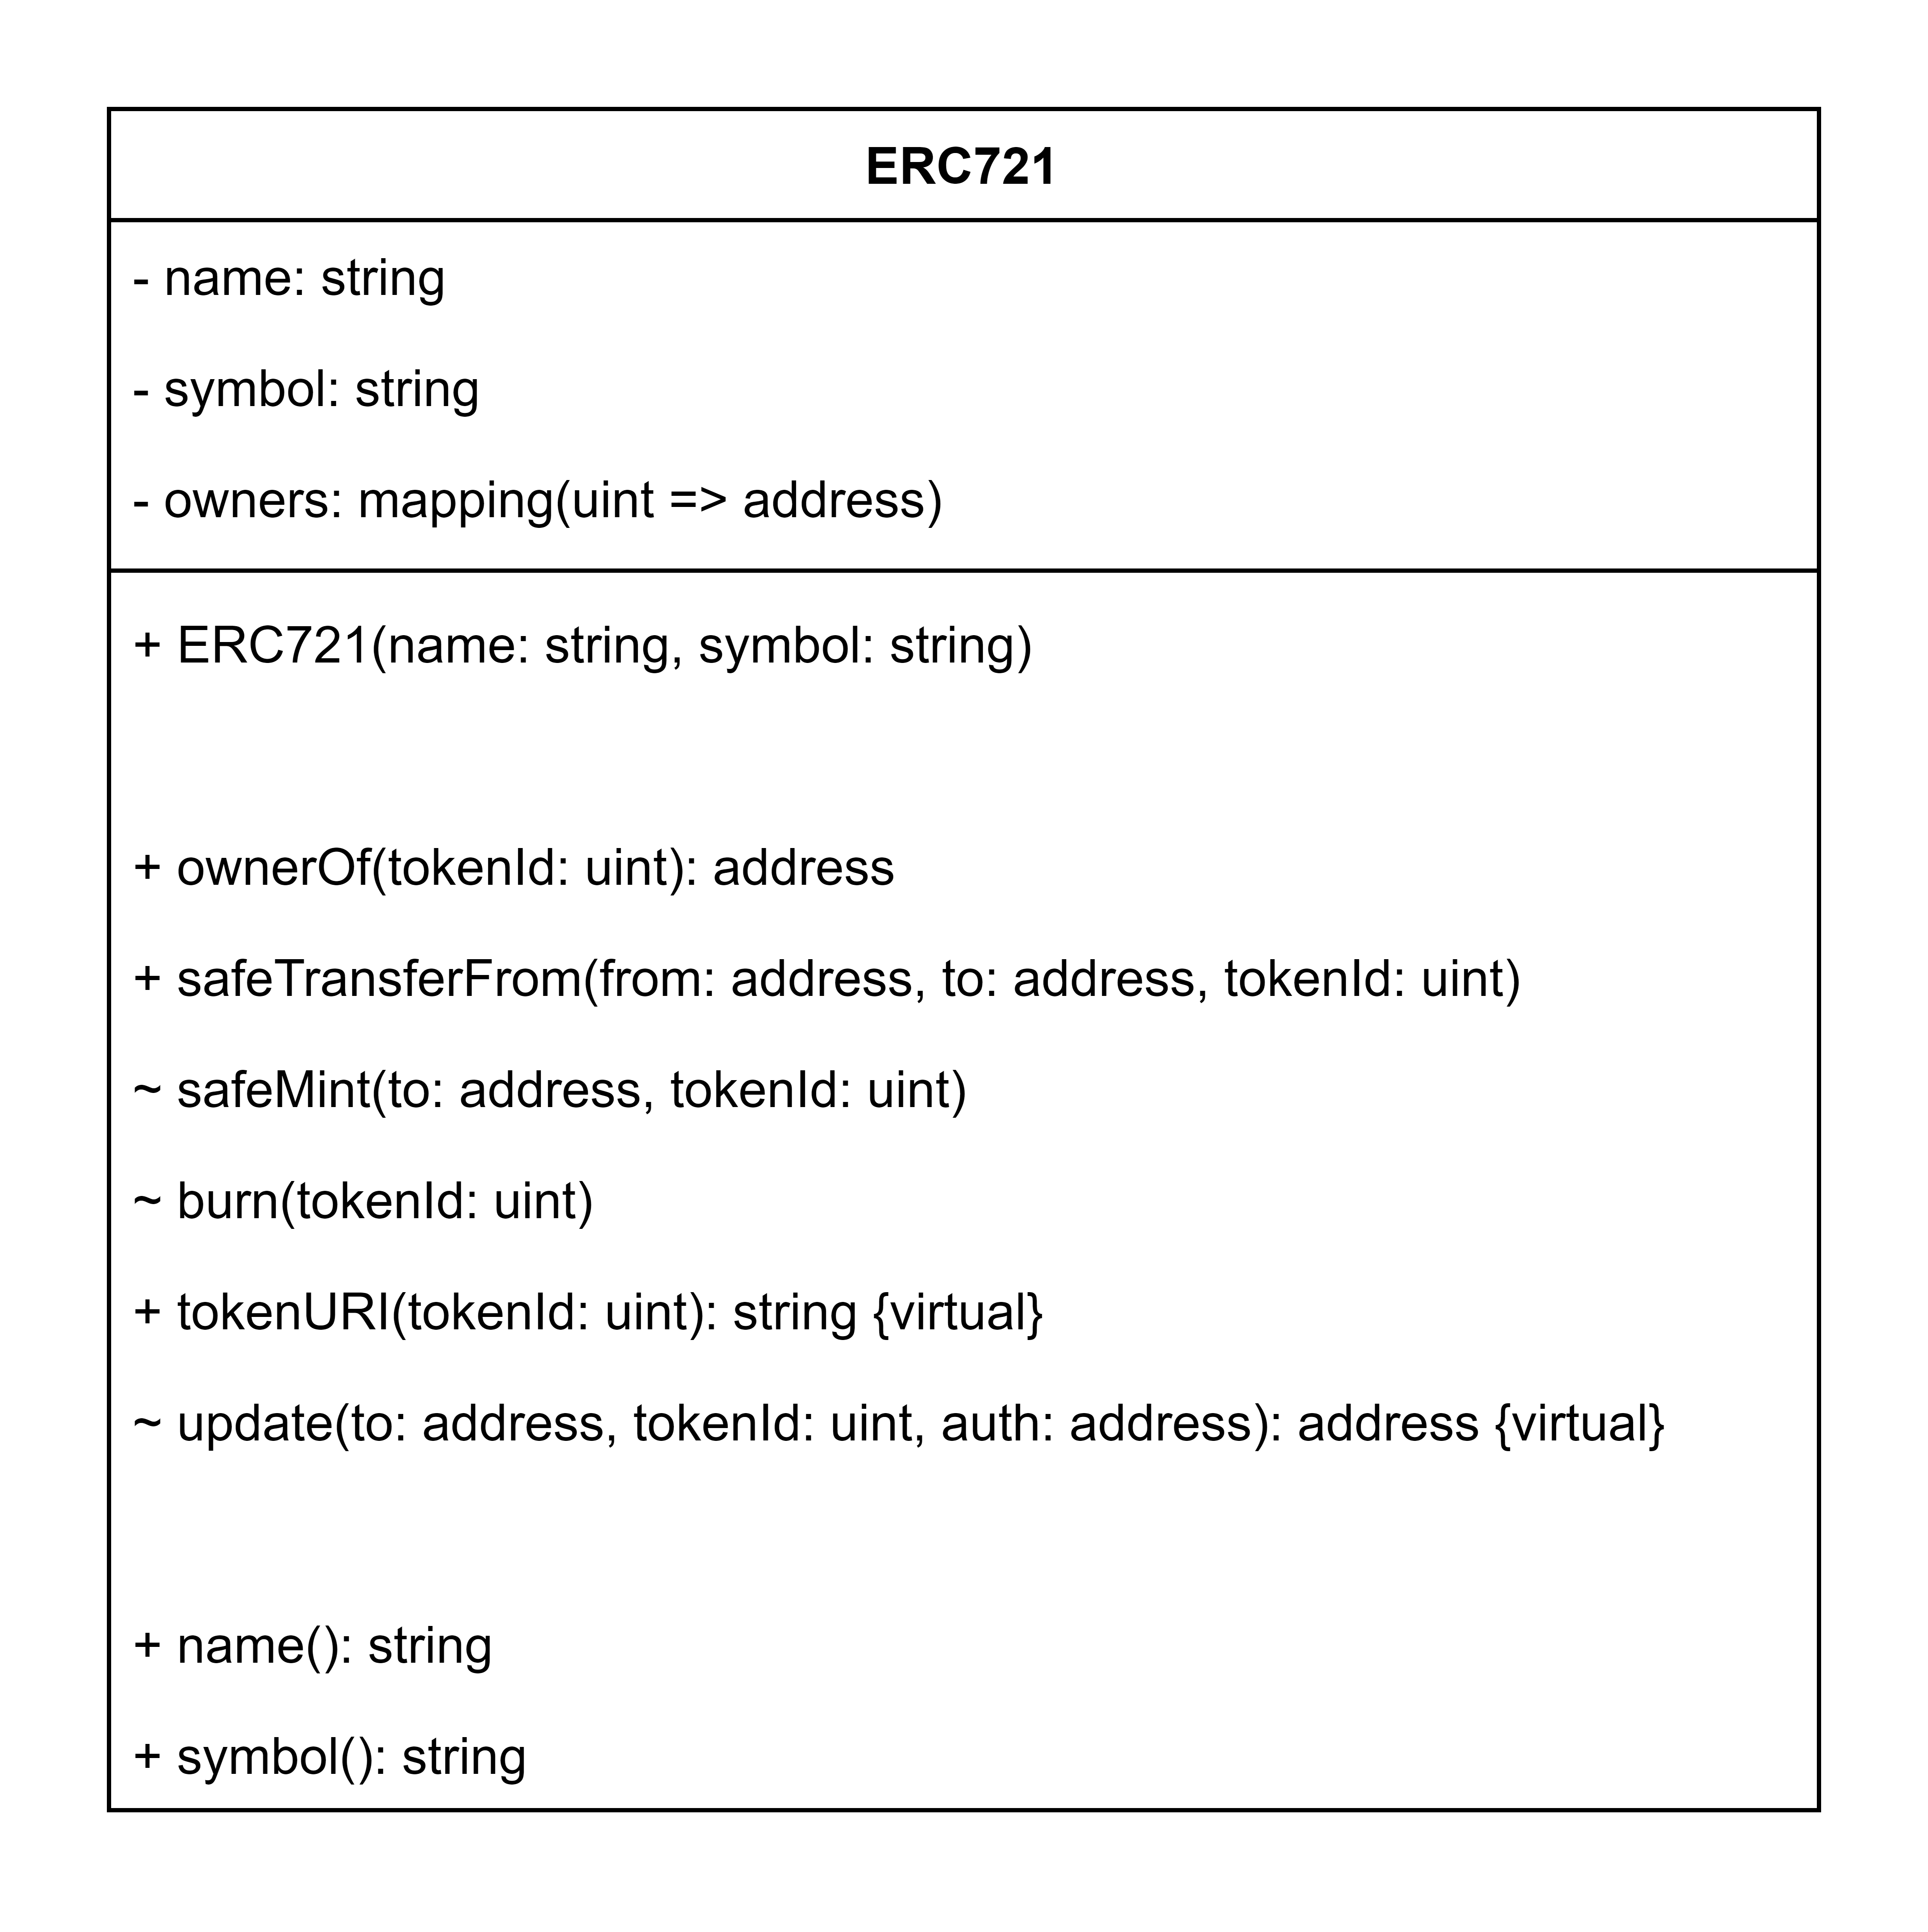
\includegraphics[width=\textwidth*2/3]{ERC721 UML.png}
	\centering
	\caption{ERC721 UML (relevant methods)}\label{fig:erc721_uml}
\end{figure}

The function \texttt{tokenURI} is the one that is called by default in the
marketplaces to get the NFT's metadata, being one of the main reasons to extend
the ERC721 standard, because it enforces the implementation of this method. In
Figure~\ref{fig:erc721_uml} we see that it has the \texttt{virtual} keyword,
meaning this can be overridden by the contracts that extend it, to manipulate
the way to store the metadata. We'll be mentioning this again in the
Section~\ref{fig:package_logic}, about how the packages logic is implemented.

\subsection{Event Contract}\label{subsec:event_contract}

So the event contract will be deployed and we need a certain control over the
tickets. One of the aspects we need to account for is that when deploying an
event, and since it will extend the ERC721 standard, any public functions on
that standard will be possible to execute. This is a problem because we don't
want the users to mint tickets whenever they want or transfer them between
themselves from outside the system, so we need to restrict these operations. As
we saw already on Figure~\ref{fig:erc721_uml}, only the
\texttt{safeTransferFrom} method is public, so users could transfer NFTs
between each other. We want that to be possible, just not from outside the
system, since that can lead users to exploit the system and scalping the
tickets easily. The minting, however, won't be an issue because it's an
internal method, so we will access it from the buy method in the event and
restrict it there.

\subsubsection{Event Lifecycle}\label{subsubsec:event_lifecycle}

The Figure~\ref{fig:event_lifecycle} shows the lifecycle of the event, and what
restrictions are in place for the ticket operations. The dates above the line
indicate the states of the event, and below a small description of the
operations that are allowed when each state is reached.

\begin{figure}[H]
	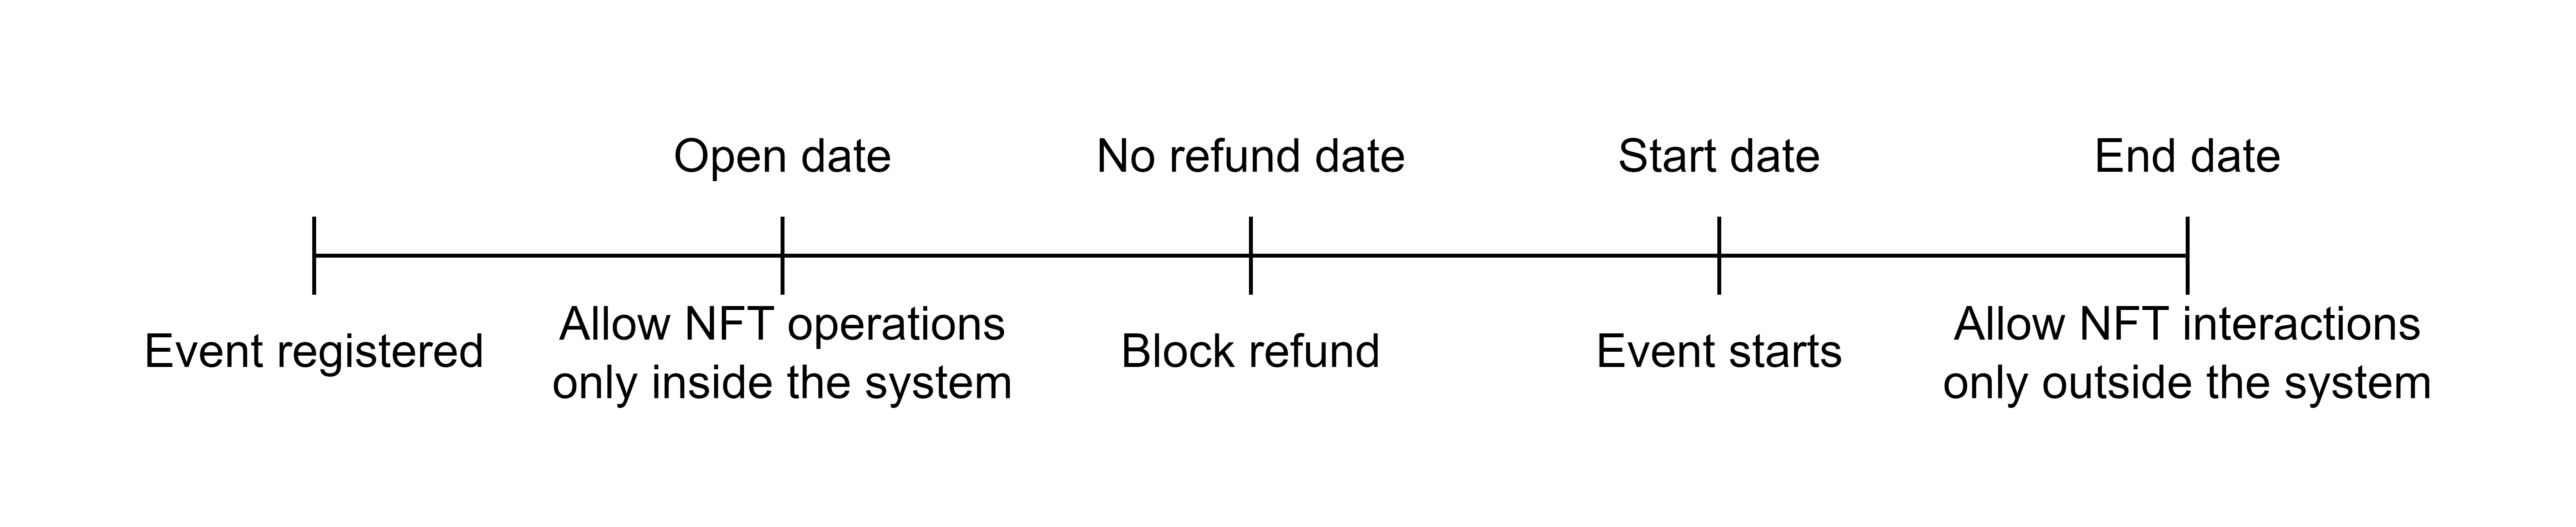
\includegraphics[width=\textwidth]{Event lifecycle.png}
	\centering
	\caption{Event lifecycle}\label{fig:event_lifecycle}
\end{figure}

We will have 4 main states for the event after it has been registered (the ones
in bold), being the \textbf{Open}, \textbf{No refund}, \textbf{Start}, and
\textbf{End} dates. Once the event is registered, it will show up in the app
for user to see, and the organizers can set a later open date to allow ticket
minting (buying).

\paragraph{Open Date:} Once it hits the \textbf{Open} date, we will allow the users to buy tickets,
which will mint the NFTs by executing the \texttt{safeMint} method of the
ERC721 standard. We will allow users to operate over the NFTs, but only within
the system. If they try to call the \texttt{safeTransferFrom} directly from the
ERC721 standard, it will revert, because we detect it's not being called
through the system.

\paragraph{No Refund Date:} After the \textbf{No refund} date, we will prevent the users to call the refund
method, which essentially \texttt{burns} the NFTs, removing them from the user
and making them available again. This is a nice operation to add because it
allows the users to get their money back if they can't attend the event. The
organizer decides the percentage of the refund and the deadline, which is there
to prevent users to buy a big amount of tickets and then refund them last
minute, which would be a way to exploit the system (in case of a 100\% refund,
they wouldn't risk anything). The other good thing for the organizer is when
the event is expected to be sold out. Since the users will get some money back,
they will have a reason to refund their tickets if they cannot attend the event
anymore, making them available again for other users to buy at the original
price, making the organizer a higher profit. After this deadline, the only
that'll be allowed is for users to resell their tickets in the system's
marketplace, which them to sell at a higher price than the refund (but never
higher than the original, of course).

\paragraph{Start Date:} The \textbf{Start} date is there to tell the users when the event starts, so
basically when the gates will open. That's the date that appears in the app, so
the users know when to show up.

\paragraph{End Date:} The \textbf{End} date tells when the event is over, unlocking all the ticket
operations to outside the system. So users can simply keep the tickets as a
souvenir or sell them in any marketplace, without any restrictions on the
tickets, including the removal of the price cap.

With this behavior in mind, we came up with the Event UML, as shown in the
Figure~\ref{fig:event_uml}, where we added the necessary methods for the
organizer/admins to manage the event and the users to handle the tickets, which
then trigger the corresponding methods of the ERC721 standard. We added a
possibility to have admins so the organizer can distribute the workload of
executing the necessary operations to people he trusts.

\begin{figure}[H]
	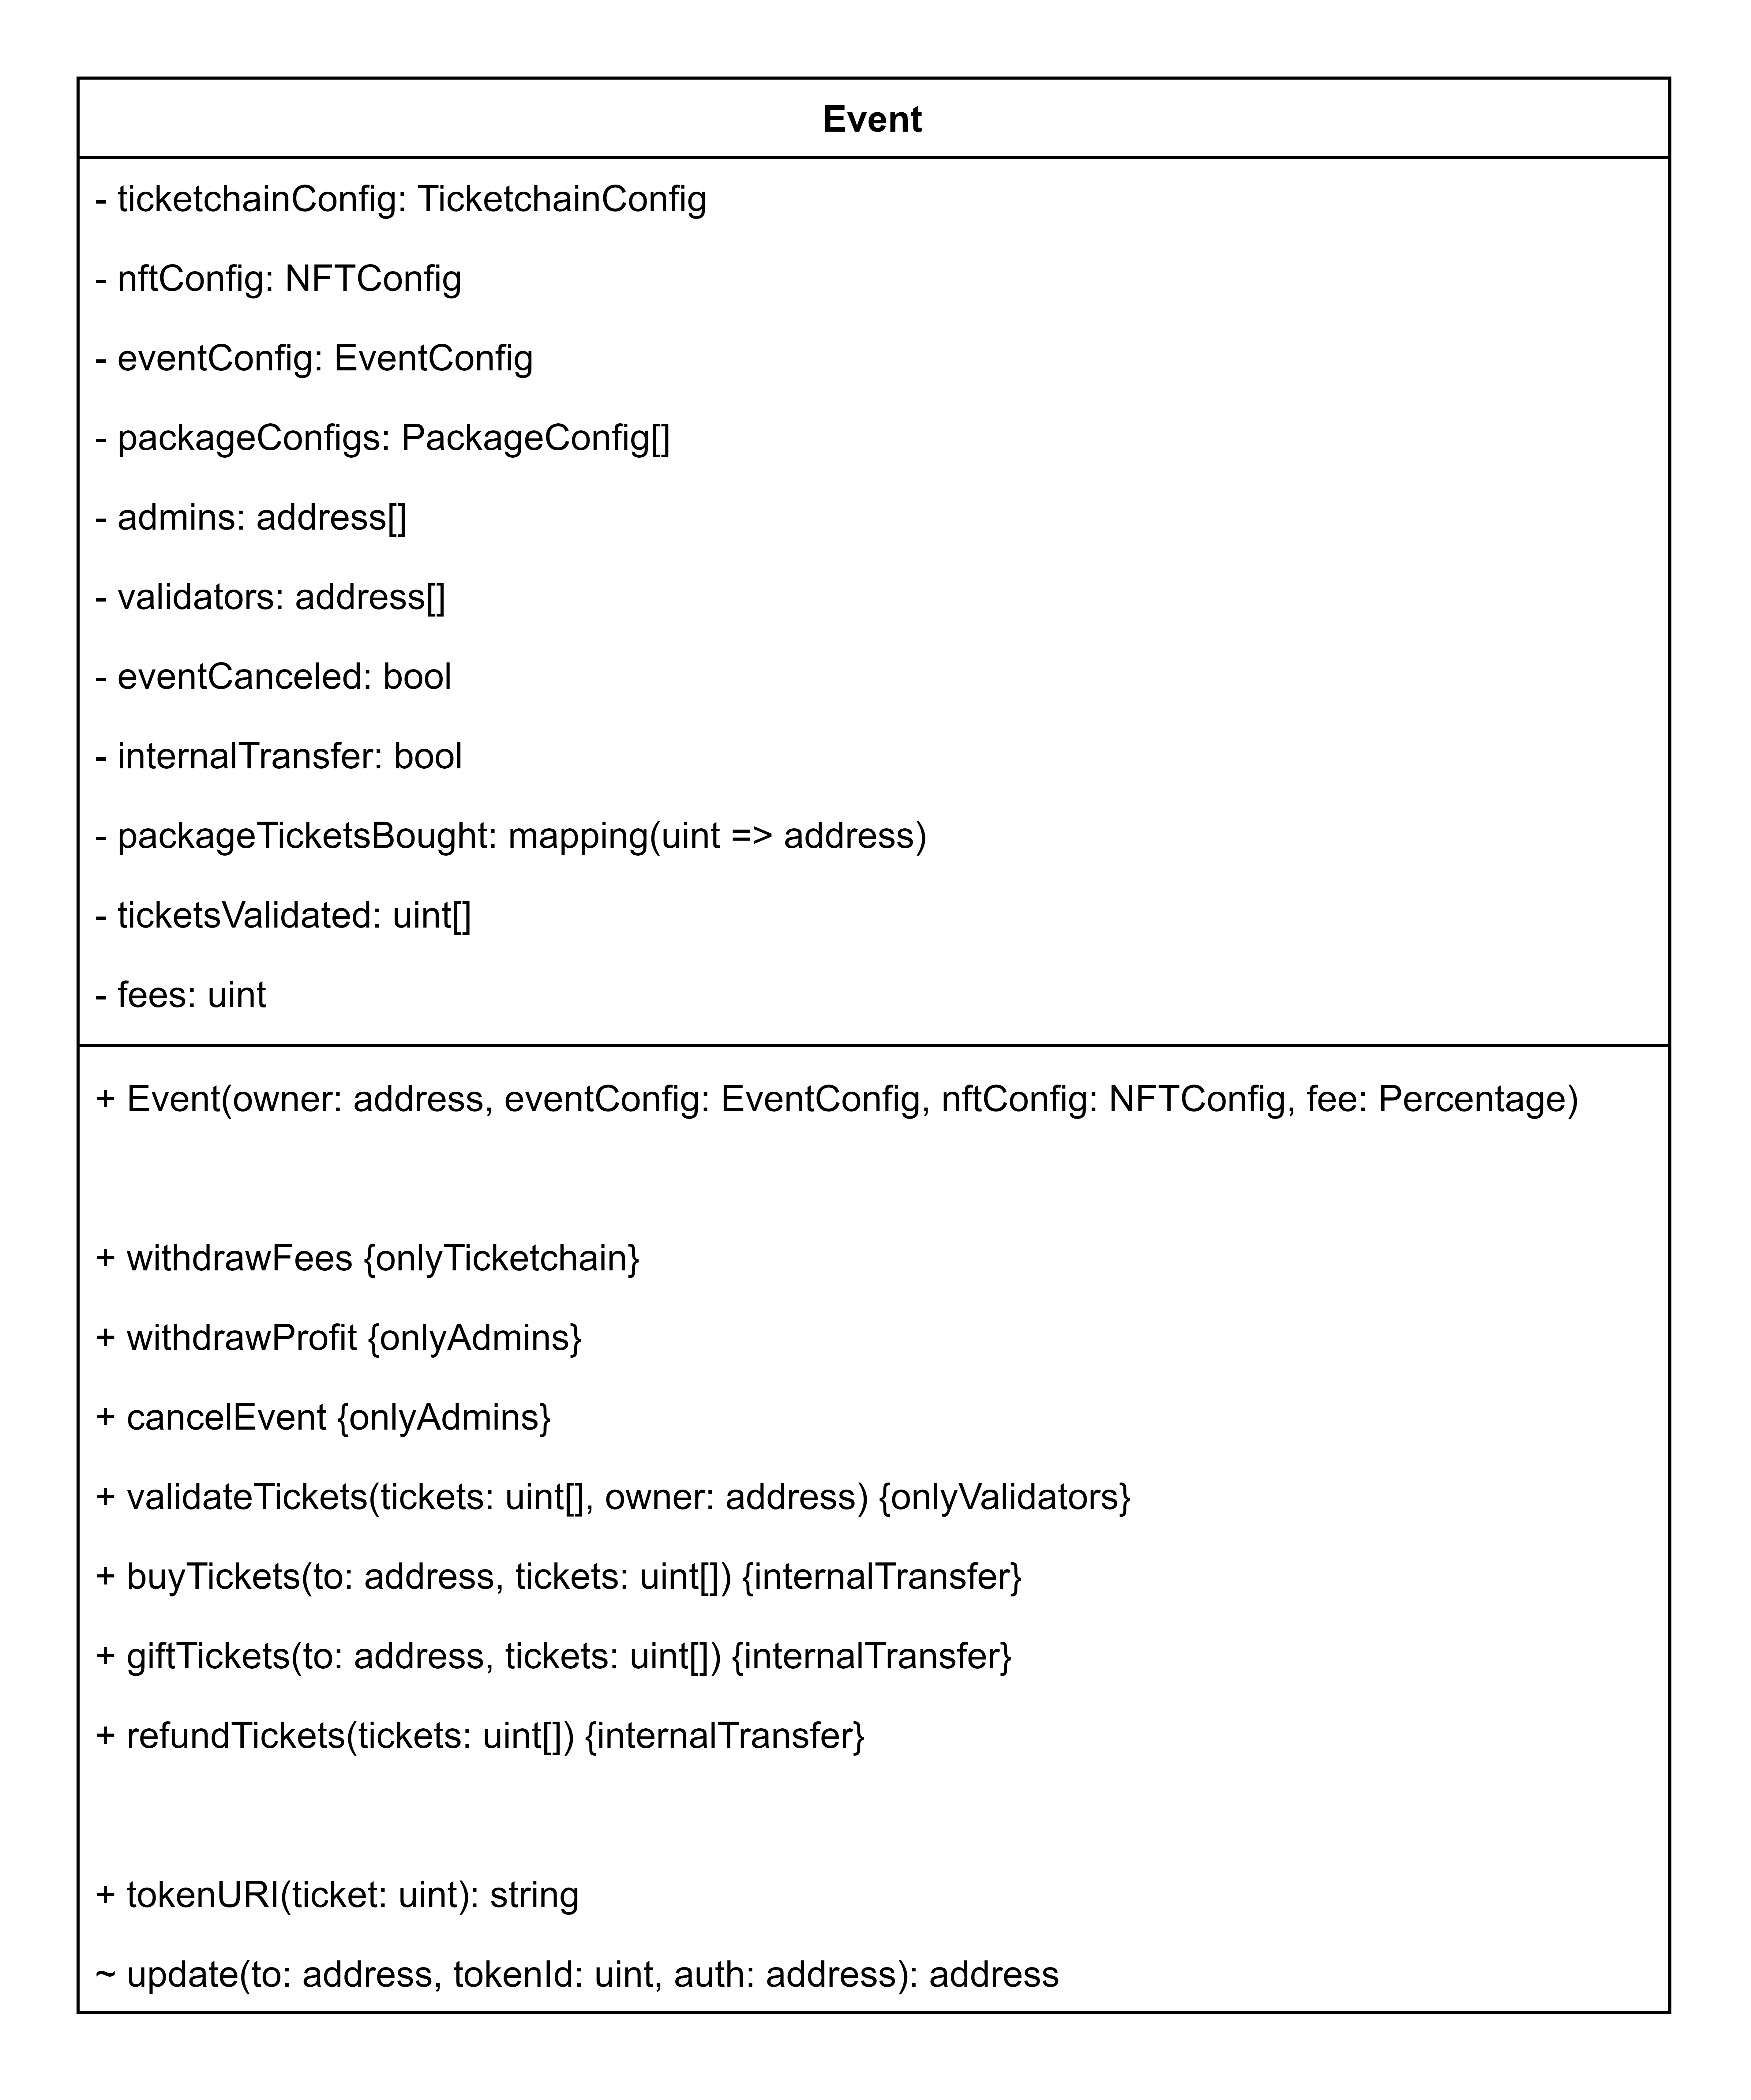
\includegraphics[width=\textwidth*3/4]{Event UML.png}
	\centering
	\caption{Event UML (relevant methods)}\label{fig:event_uml}
\end{figure}

As we can see, the \texttt{update} method has been overridden from the ERC721
standard to restrict the interactions with the NFTs according the defined
behavior. This method is the one that gets called anytime there's an operation
on any NFT, so we can implement here the necessary logic to restrict the
operations, and we can visualize that in the flowchart shown in
Figure~\ref{fig:nft_flowchart}.

\begin{figure}[H]
	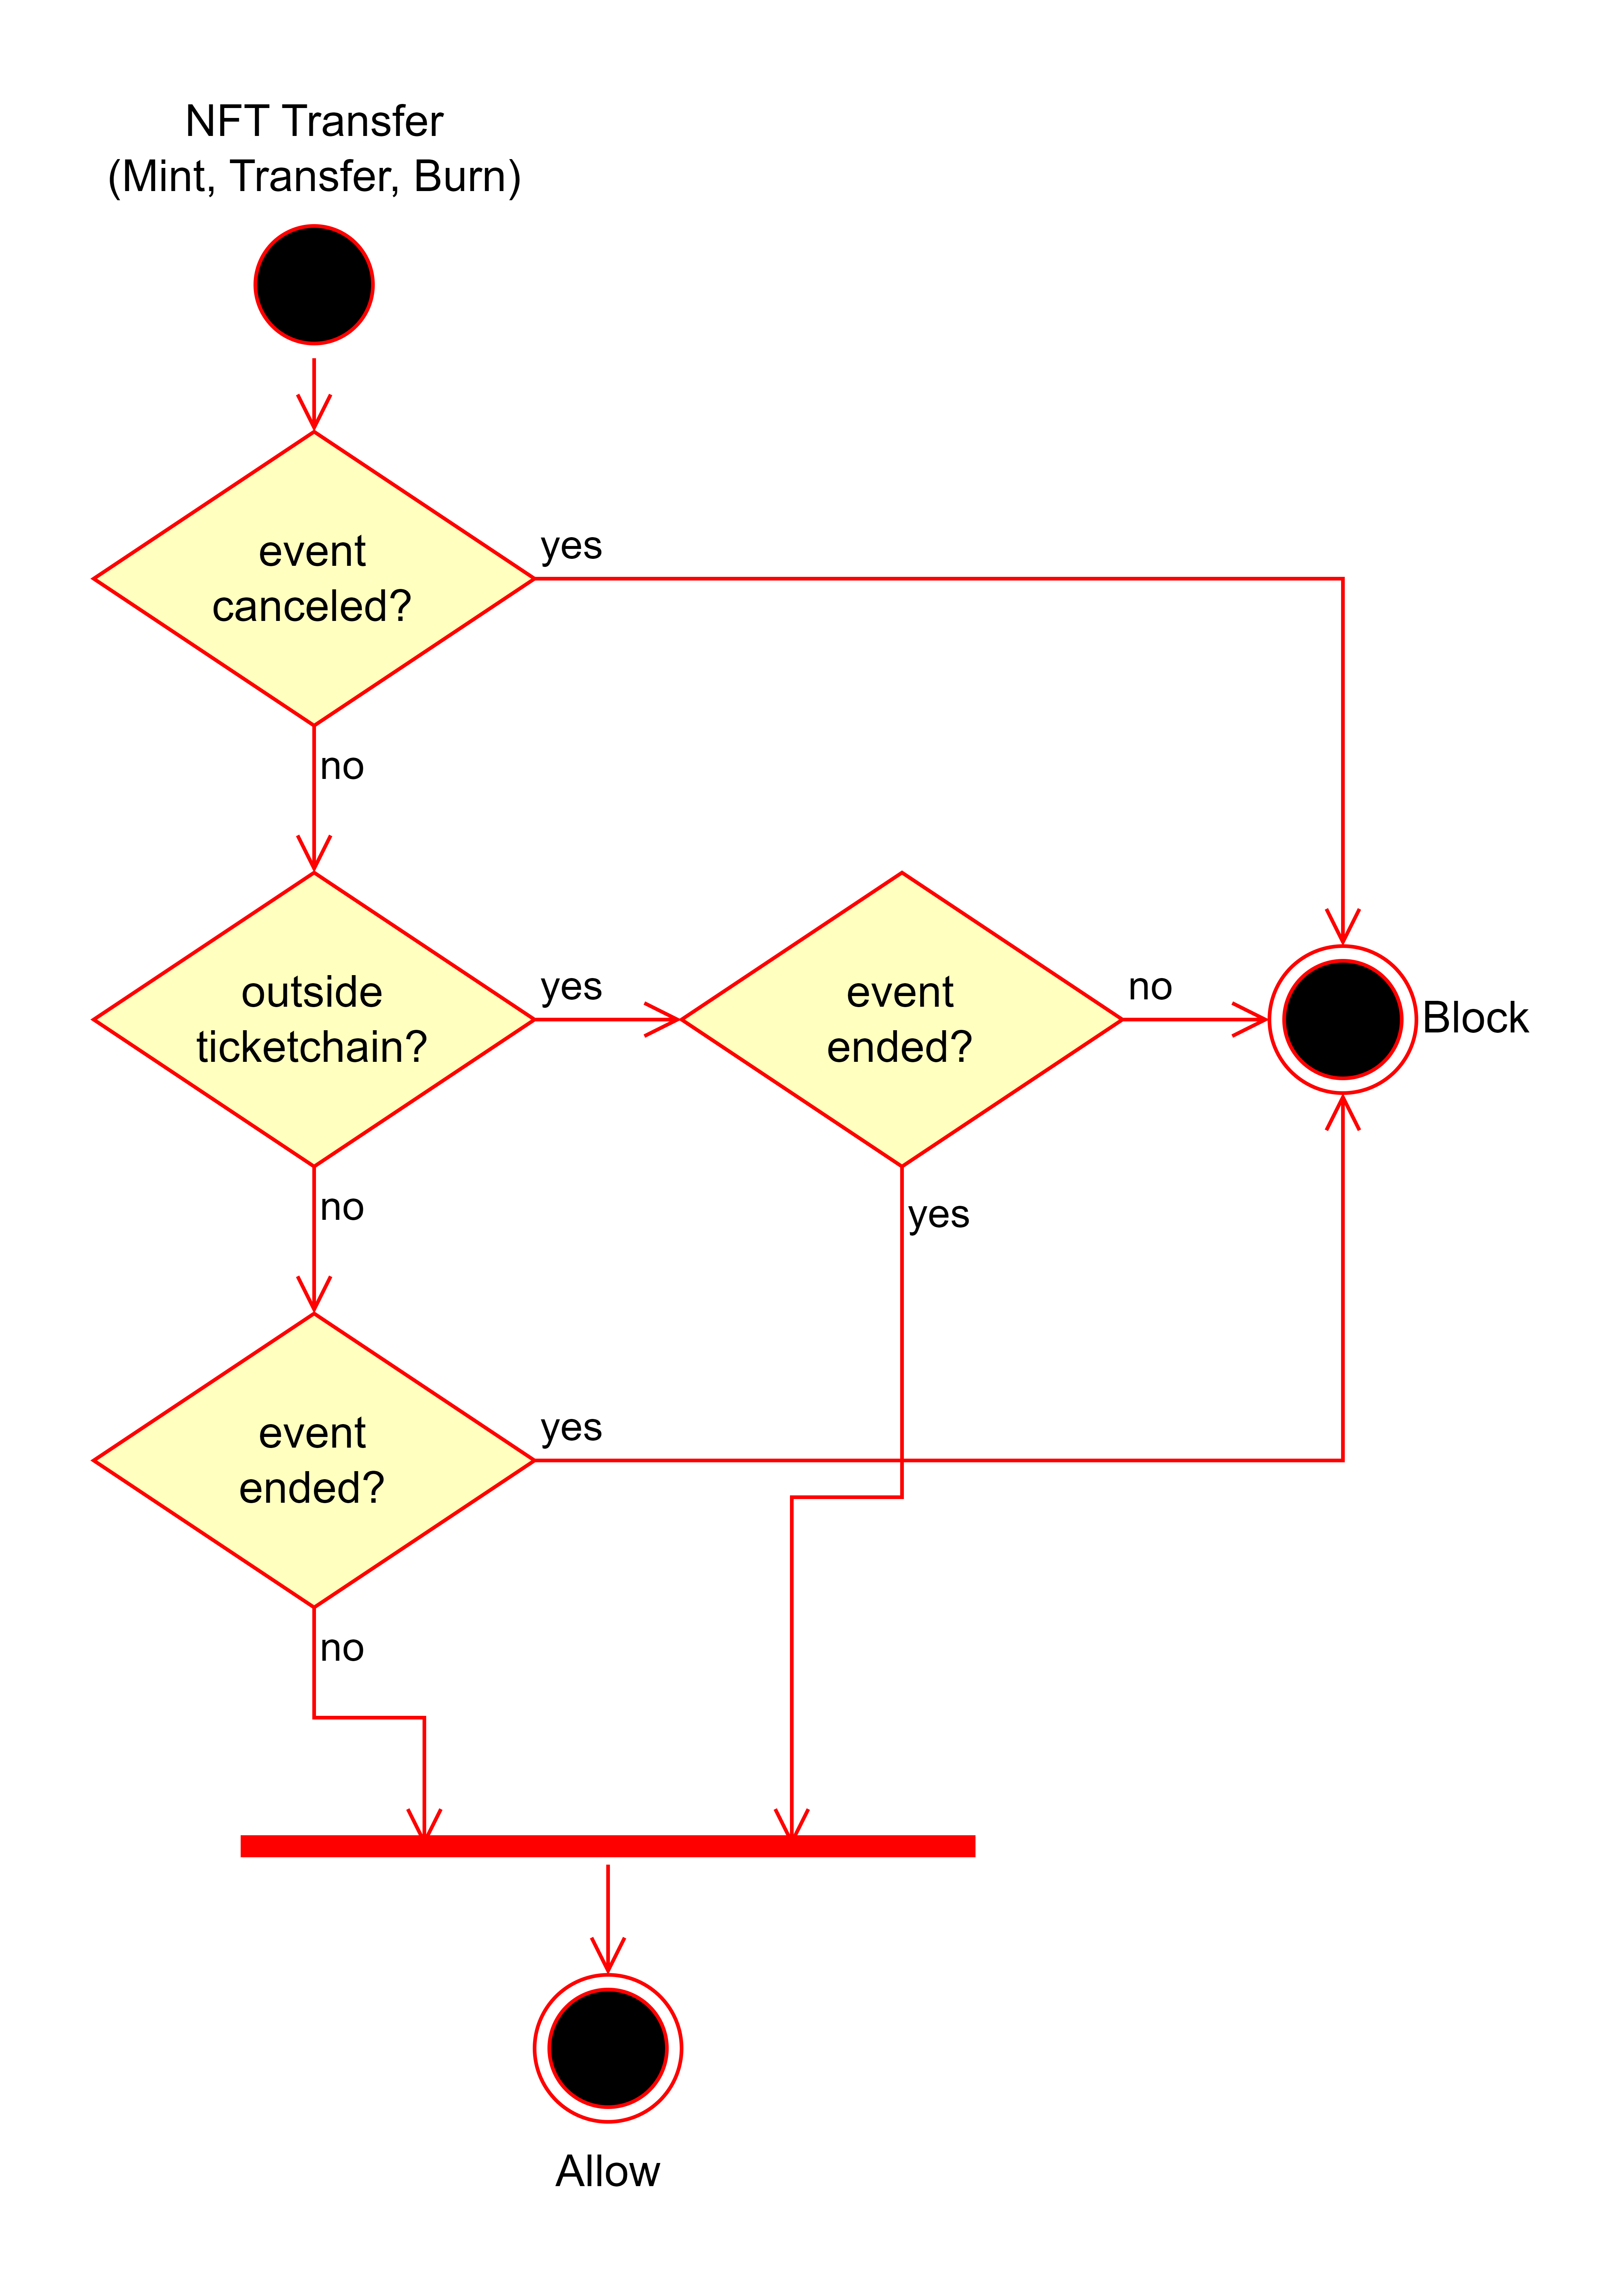
\includegraphics[width=\textwidth*2/3]{NFT flowchart.png}
	\centering
	\caption{NFT flowchart}\label{fig:nft_flowchart}
\end{figure}

This logic is possible to implement because of modifiers, mentioned before.
What we essentially do on that modifier, is set a variable to true (meaning the
NFT operation is coming from within the system), execute the function it's
assigned to, and then we set the variable back to false. Then we apply that
modifier on the necessary functions, which we can see them with the operator
	{internalTransfer} in the event UML, shown in Figure~\ref{fig:event_uml}.

\subsubsection{Structs}\label{subsubsec:structs}

From Figure~\ref{fig:ticketchain_uml} and Figure~\ref{fig:event_uml}, the UML
of our smart contracts, we can see that we have a few custom structs to better
organize the data. These structs are the \texttt{Percentage},
\texttt{EventConfig}, \texttt{NFTConfig}, \texttt{PackageConfig} and
\texttt{TicketchainConfig} structs.

\paragraph{Percentage Struct:} The \texttt{Percentage} struct is necessary because in Solidity there are no
floating point numbers, so we need a way to make calculations with percentages.
What this struct does is it stores the value of the percentage and the amount
of decimals it has, so if we want to calculate 55.50\% of a number, we would
have 555 as the value with 1 decimal, or 5550 with 2 decimals. The struct is
shown in Listing~\ref{lst:percentage_struct}:
\begin{lstlisting}[caption=Percentage struct,label={lst:percentage_struct}]
struct Percentage {
	uint256 value;
	uint256 decimals;
}
\end{lstlisting}
so to obtain a percentage of some $x$ number, we do $y = \frac{x \times
		\text{Percentage.value}}{100\mathrm{e}^\text{Percentage.decimals}}$.

When working with ether units, it can be common to have values like 0.00005
ether, but it's rather rare to have values in wei like 1000 wei, so applying
this formula won't lose much precision (note that 1 ether is $10^{18}$ wei).
Equating this to real world value, 0.001 ether is somewhat close to 2.5\$ (at
the moment), so 1000 wei would be way lower than even a cent.

\paragraph{TicketchainConfig Struct:} The \texttt{TicketchainConfig} struct is simply to keep it stored the system
address and the system fee percentage, so we can easily access this information
when applying the fees and withdrawing them, and is shown in
Listing~\ref{lst:ticketchain_config_struct}:
\begin{lstlisting}[caption=TicketchainConfig struct,label={lst:ticketchain_config_struct}]
struct TicketchainConfig {
    address ticketchainAddress;
    Percentage feePercentage;
}
\end{lstlisting}

\paragraph{NFTConfig Struct:} The \texttt{NFTConfig} struct is just to store the NFTs basic information, like
the name, symbol, and base URI, to ease the input of the NFTs information when
registering the event, as Listing~\ref{lst:nft_config_struct} shows:
\begin{lstlisting}[caption=NFTConfig struct,label={lst:nft_config_struct}]
struct NFTConfig {
	string name;
	string symbol;
	string baseURI;
}
\end{lstlisting}
The \texttt{name} is the name of the NFT collection and the symbol is the
abbreviation of it, like the name being \textit{Ticketchain} and the symbol
being \textit{TCK}, for example. The base URI is the link to the metadata of
the NFTs, which will be used to get the information about the tickets.

\paragraph{EventConfig Struct:} The \texttt{EventConfig} struct is to store the event's entire configuration,
like the name, description, location, dates, and refund, as shown in
Listing~\ref{lst:event_config_struct}:
\begin{lstlisting}[caption=EventConfig struct,label={lst:event_config_struct}]
struct EventConfig {
	string name;
	string description;
	string location;
	uint256 openDate;
	uint256 noRefundDate;
	uint256 startDate;
	uint256 endDate;
	Percentage refundPercentage;
}
\end{lstlisting}

\paragraph{PackageConfig Struct:} Lastly, the \texttt{PackageConfig} struct is there to store each package
information, to keep track of the ones that are available for the event, as
Listing~\ref{lst:package_config_struct} shows:
\begin{lstlisting}[caption=PackageConfig struct,label={lst:package_config_struct}]
struct PackageConfig {
	string name;
	string description;
	uint256 price;
	uint256 supply;
	bool individualNfts;
}
\end{lstlisting}
This structure will be better discussed in the next Section.

\subsubsection{Ticket Packages}\label{subsubsec:ticket_packages}

It's common to see events with different types of tickets, like VIP, standard,
or even 3-day passes, each with its own price and benefits. We want to
implement this feature in the system, so we can have a better control over the
tickets and the users can choose the one that fits them better.

For that, we will allow the organizer to add packages, indicating the supply of
each one, and as we saw already, the NFTs are a mapping of the ID to the owner,
so we can organize the packages as a list, where the supply and order of them
assigns the ID of each NFT to the package, like the
Figure~\ref{fig:package_logic} illustrates.

\begin{figure}[H]
	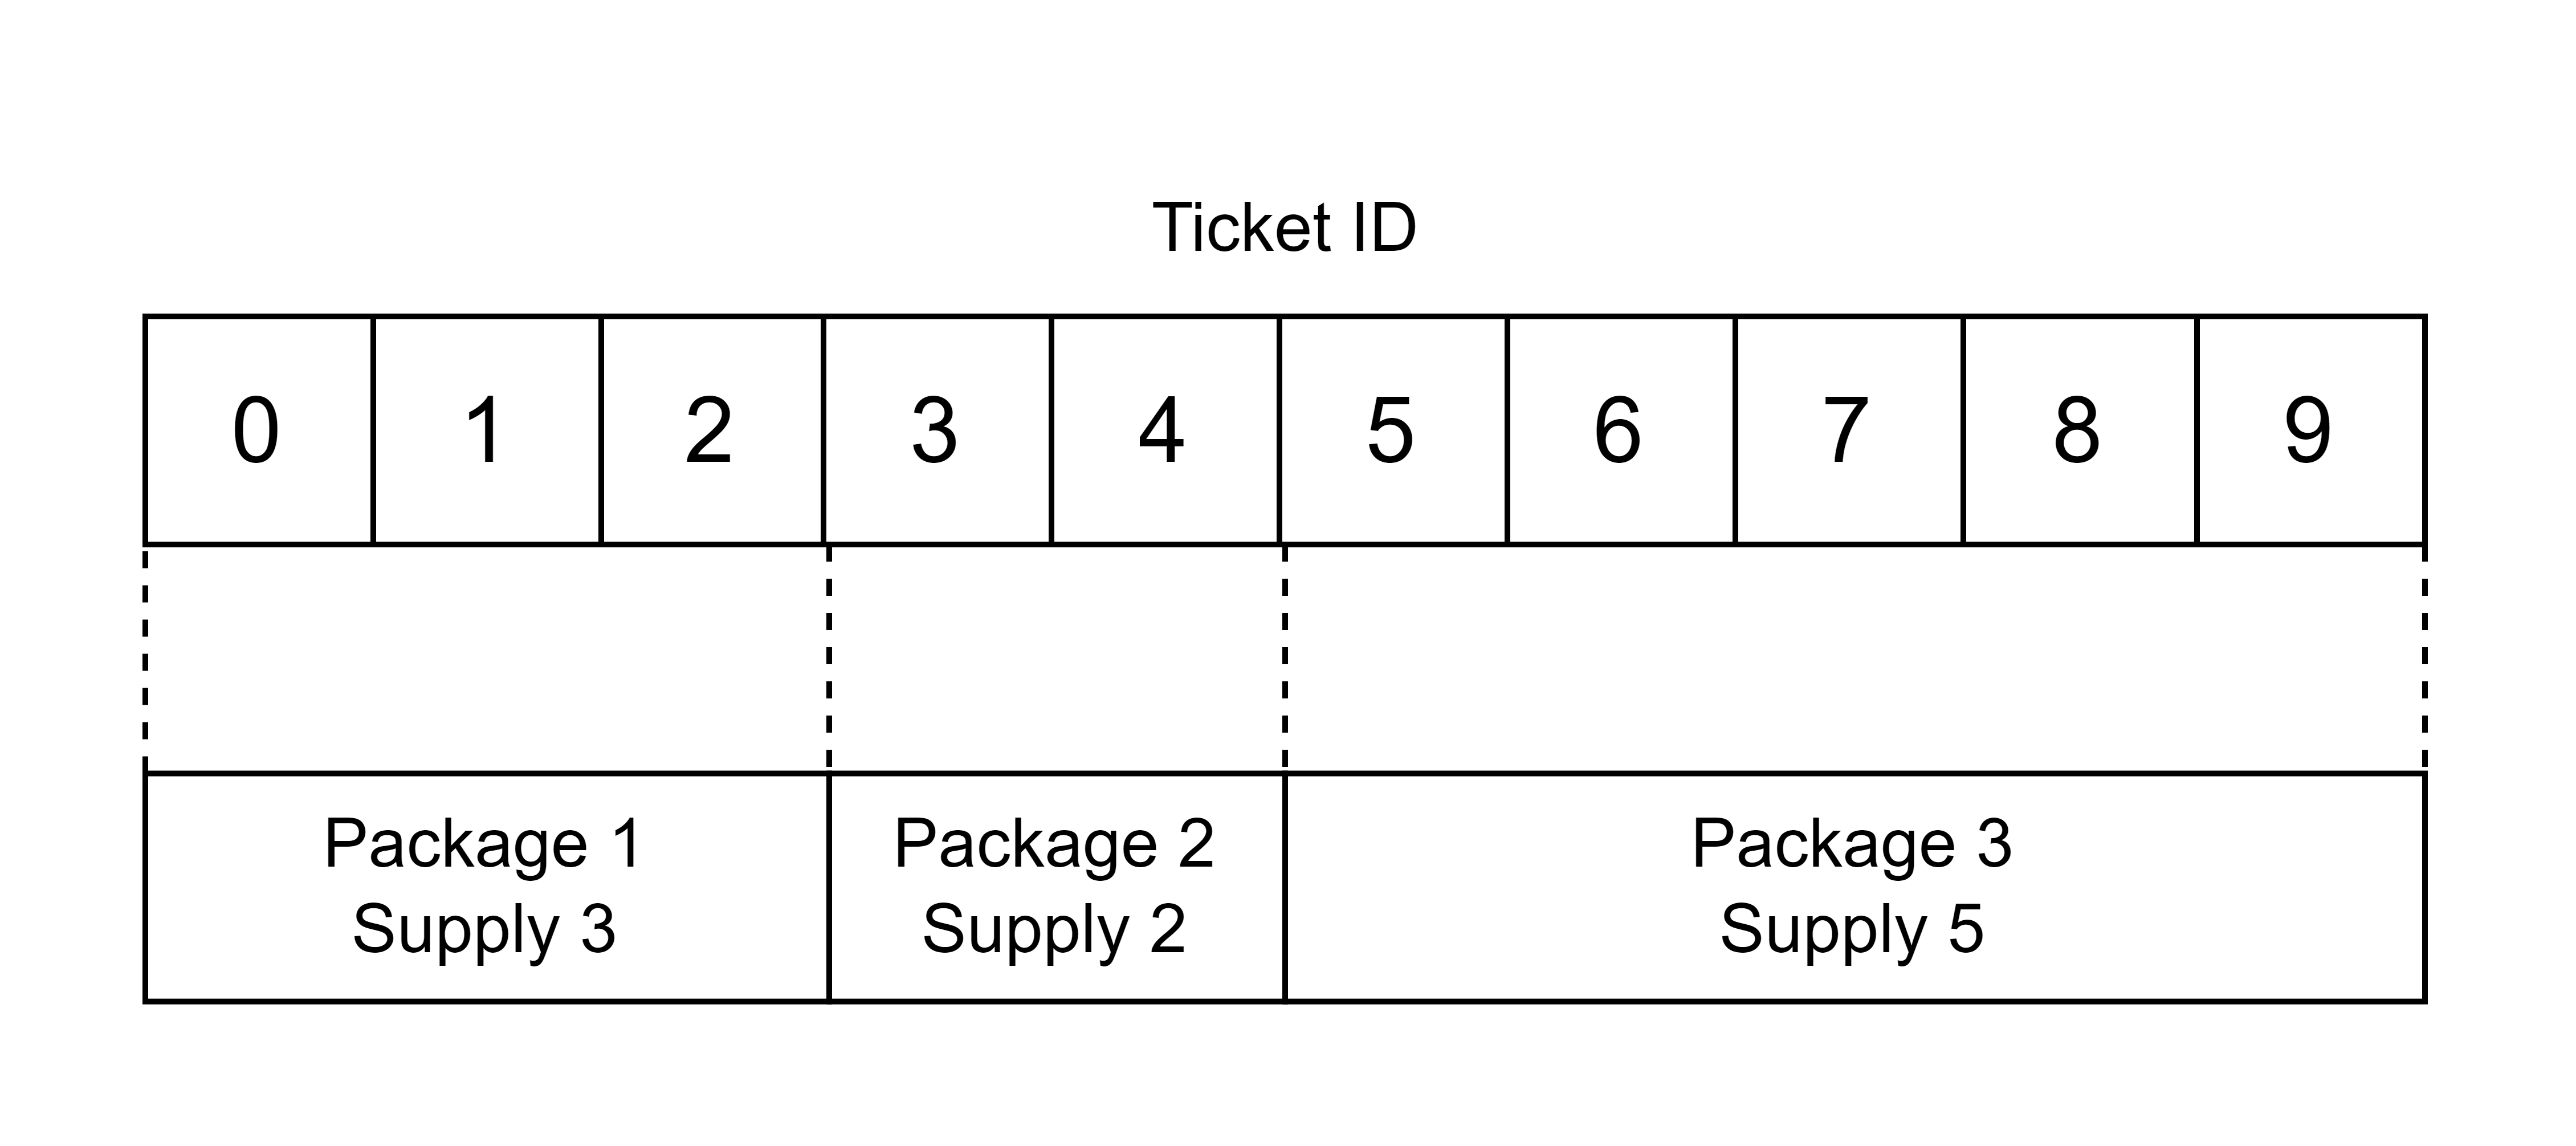
\includegraphics[width=\textwidth*2/3]{Package logic.png}
	\centering
	\caption{Package logic}\label{fig:package_logic}
\end{figure}

This way, whenever we need to get a ticket for a certain package, we can go
through the packages and see which one the ID is in. One only limitation with
this is if the event is already open (users can buy tickets), the only thing we
can allow the organizer to do is to add packages, neither remove or change
their order, because that would change the package associated to the tickets,
which would be a problem for the users that already bought them.

Now we just have to make sure the information obtained with the
\texttt{tokenURI} method corresponds to the ticket, according to its package.
For this we will have a different metadata file for each package, with the
necessary information about the tickets. The \texttt{individualNfts} boolean in
the \texttt{PackageConfig} struct is there to indicate if the organizer wants
each ticket on the package to have its own metadata, or if they can share it.

According to this, the \texttt{tokenURI} will return an URI like
\texttt{baseURI/packageId/ticketId} for a package with individual NFTs, and
\texttt{baseURI/packageId} for a package with shared metadata. Like this, when
we store the metadata on the \gls{ipfs}, we store the metadata for each ticket
inside a folder of the packages with individual NFTs, and only a metadata file
for each package without individual NFTs.

\subsubsection{Metadata Storage}\label{subsubsec:metadata_storage}

To store the NFTs metadata files, we'll be using the \gls{ipfs} for storing the
NFTs metadata. The \gls{ipfs} is a decentralized storage system where the data
is stored in a distributed network of nodes (decentralized), making it very
secure and reliable. This is a good solution for storing the metadata of the
NFTs because it's very cheap and easy to use, and it's a common practice in the
blockchain ecosystem.

Other options would be to store the data on some kind of server, but that would
be more expensive to maintain, and since we are dealing with NFTs, it's good
practice to store the data in a decentralized manner, to avoid any kind of
alteration on its contents, if the tickets possibly become valuable
collectibles.

This kind of issue was something that has happened before, where people bought
NFTs with the idea of them being somewhat valuable, but then the owner changed
the contents of the metadata, executing what was called of a \textit{rug pull},
which is a scam that made the NFTs worthless, keeping the money for himself.

To store the data on the \gls{ipfs}, we will be using the Pinata~\cite{pinata}
service, which does the heavy lifting for interacting with the storage itself.
To accomplish this, we just need to arrange the files according to the ticket
packages, like mentioned before in the Section~\ref{subsubsec:ticket_packages},
and then upload them to the \gls{ipfs}, getting the link to the metadata, which
we'll then store on the contract as the base URI. The files would be stored
like Figure~\ref{fig:metadata_storage} shows, being the packages 1 and 3 with
shared metadata, and the package 2 with individual NFTs.

\begin{figure}[H]
	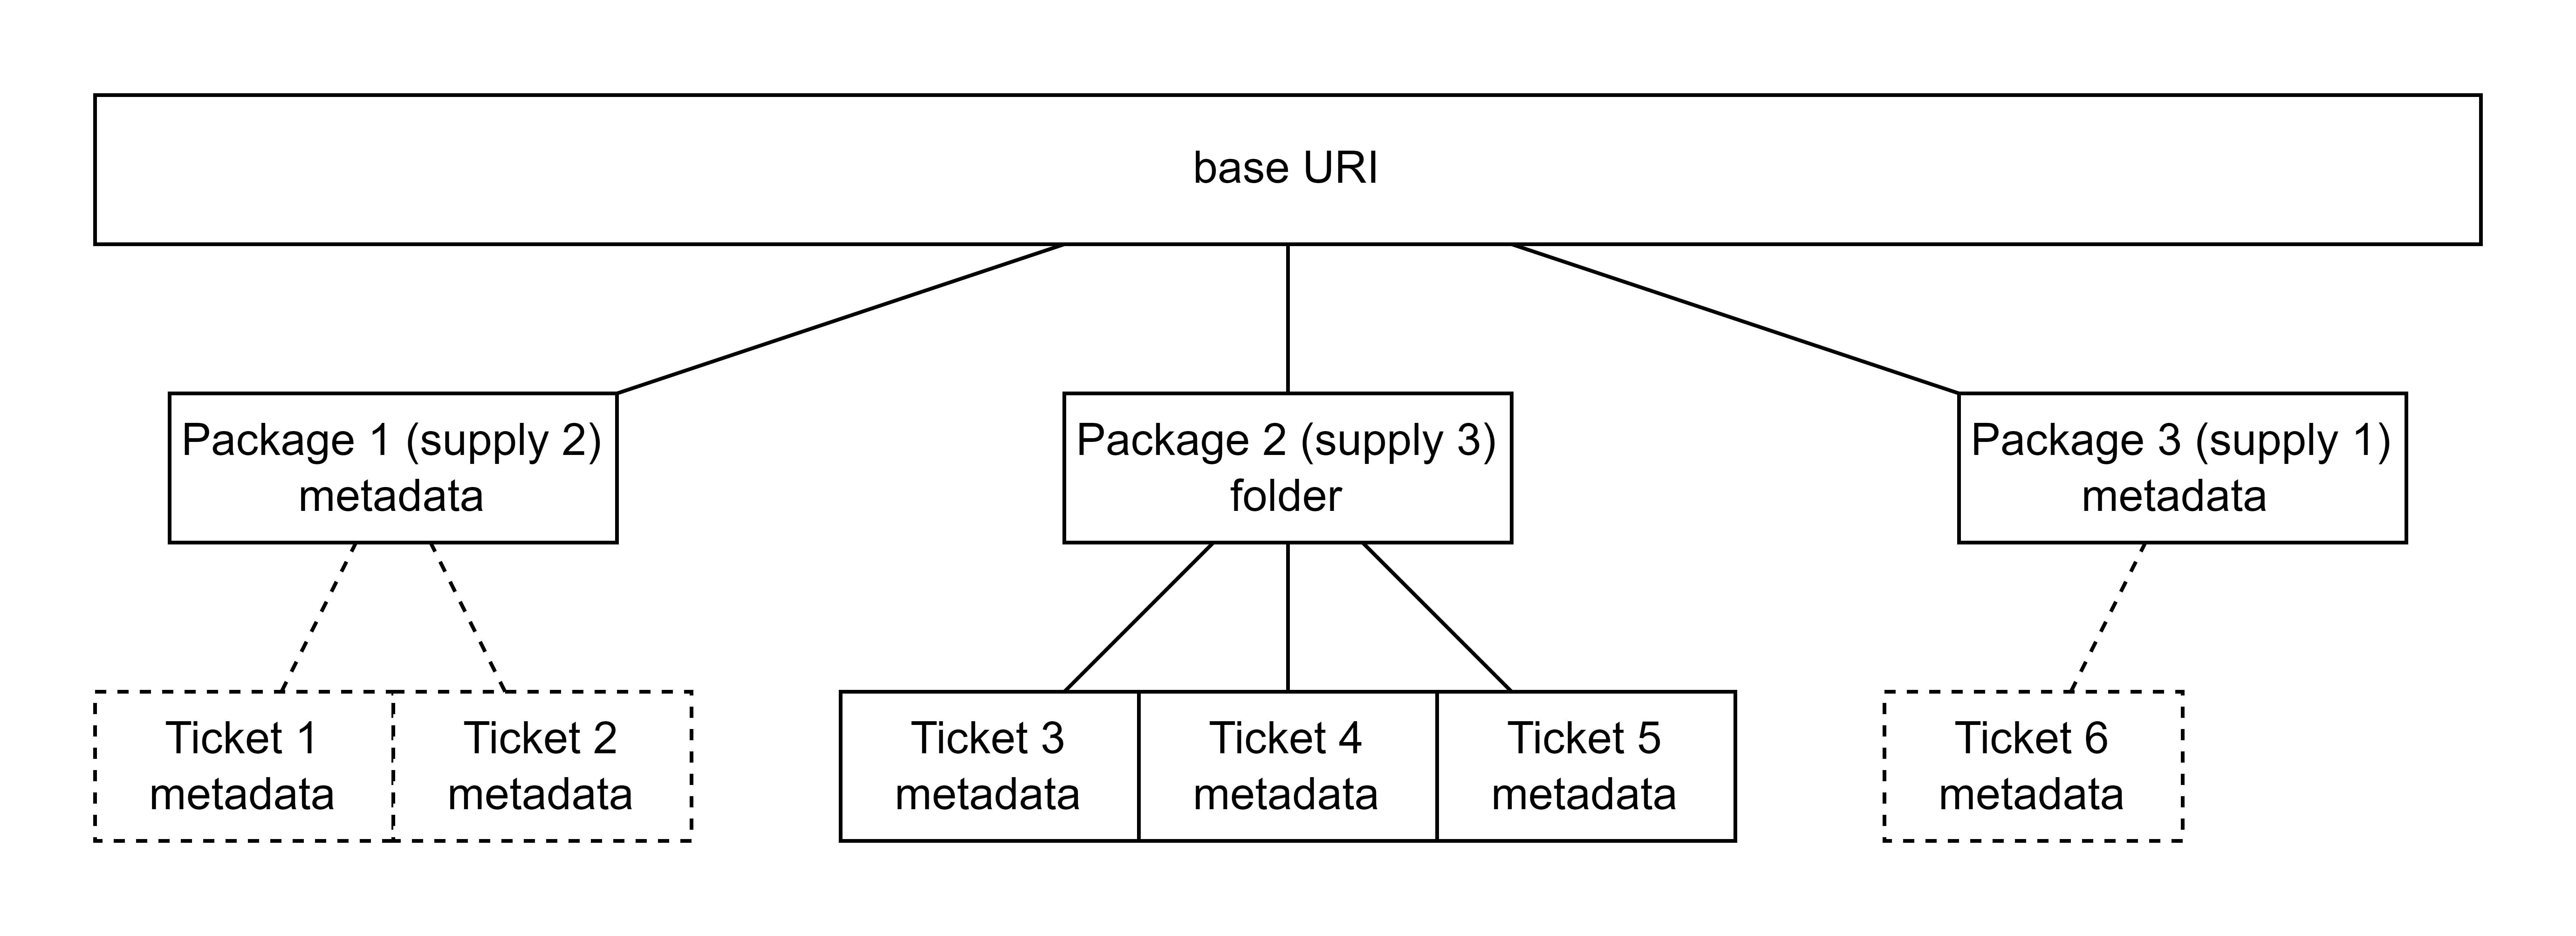
\includegraphics[width=\textwidth]{Metadata storage.png}
	\centering
	\caption{Metadata storage}\label{fig:metadata_storage}
\end{figure}

\subsubsection{System Fees}\label{subsubsec:system_fees}

One of the most important aspects of a system like this is the business model
we have to take into account. Since this is a service we want to deploy for
event organizers, we need to make this sustainable and profitable. This kind of
service aims to do some heavy lifting, with its own features, so we could set a
fee lower than the usual on the traditional marketplaces and ticket selling
platforms, since the organizers need to pay for each service.

These low fees are possible because with the system being deployed on the
blockchain, it stays there while the network is running, so the only extra cost
are the network fees (also called gas fees) when interacting with the event.
For the users, each interaction is paid by them, so when a user buys a ticket,
the only thing to take into account are the network fees, which depending on
the network, can be super low.

The other kind of fee the organizer needs to look out for is for the validators
to validate the tickets, which is a necessary operation to avoid people from
exploiting the system. These fees are paid by the validators, which the
organizer essentially manages, so we need to take them into account when
setting the system fee, to make it sustainable for the organizer to use our
system, since the organizers will have to funds the validators' wallets.

We'll set a fee on the Ticketchain smart contract, where will be stored in the
event when registering it, so that if we decide to change it, the previous
events aren't affected. This is also because we want to abstract the user of
any extra fee, so the price the organizer sets, is the price the user pays, and
the system fee is taken from the ticket price. In case an event gets cancelled,
or a user decides to get a refund, the ticket fee is returned to the user
(proportional to the refund), making the system less profit, but guarantees the
users of a fair process. With this, we need to restrict the system to only
withdraw any profit after the event is over. Since this is rather an uncommon
case, the less profit that the system makes, possibly compensates for the trust
that the users and organizers will have on it.
